%Este trabalho está licenciado sob a Licença Creative Commons Atribuição-CompartilhaIgual 3.0 Não Adaptada. Para ver uma cópia desta licença, visite http://creativecommons.org/licenses/by-sa/3.0/ ou envie uma carta para Creative Commons, PO Box 1866, Mountain View, CA 94042, USA.

\documentclass[main.tex]{subfiles}

\begin{document}

\chapter{Derivação e integração numérica}

\section{Derivação Numérica}\index{derivação numérica}

Dado um conjunto de pontos $(x_i,y_i)_{i=1}^n$, a derivada $\left(\frac{dy}{dx}\right)_i$ pode ser calculada de várias formas. Na próxima seção trabalharemos com diferenças finitas, que é mais adequada quando as abcissas estão próximas e os dados não sofrem perturbações significativas. Na seção subsequente trataremos os casos quando os dados oscilam via ajuste ou interpolações de curvas.

\subsection{Aproximação da derivada por diferenças finitas}\index{fórmula de diferenças finitas}

A derivada $f'(x_0)$ de uma função $f(x)$ no ponto $x_0$ é
\begin{equation*}
  f'(x_0)=\lim_{h\to 0}\frac{f(x_0+h)-f(x_0)}{h}.  
\end{equation*}
Da definição, se $h\neq 0$ é pequeno (não muito pequeno para evitar o cancelamento catastrófico), é esperado que uma aproximação para a derivada no ponto $x_0$ seja dada por:
\begin{equation}\label{eq:dp}
  f'(x_0)\approx \frac{f(x_0+h)-f(x_0)}{h}.  
\end{equation}

\begin{ex}\label{ex:dp}
Calcule a derivada numérica da função $f(x)=\cos(x)$ no ponto $x=1$ usando $h=0,1$, $h=0,01$, $h=0,001$ e $h=0,0001$.
\end{ex}
\begin{sol}
Usando a fórmula de diferenças dada pela Equação~\eqref{eq:dp}, devemos calcular:
\begin{equation*}
  f'(x) \approx \frac{cos(1 + h) - cos(1)}{h}
\end{equation*}
para cada valor de $h$ solicitado. Fazendo isso, obtemos a seguinte tabela:
\begin{equation*}
\begin{array}{|c|c|}
\hline
\vspace{-10pt}&\\
h & \dfrac{f(1+h)-f(1)}{h} \\
\vspace{-10pt}&\\
\hline
\vspace{-10pt}&\\
0,1 & \dfrac{0,4535961-0,5403023}{0,1}=- 0,8670618\\
\vspace{-10pt}&\\
\hline
\vspace{-10pt}&\\
0,01 & \dfrac{0,5318607-0,5403023}{0,01}=- 0,8441584\\
\vspace{-10pt}&\\
\hline
\vspace{-10pt}&\\
0,001 & \dfrac{0,5403023-0,5403023}{0,001}=- 0,841741\\
\vspace{-10pt}&\\
\hline
\vspace{-10pt}&\\
0,0001 & \dfrac{0,5403023-0,5403023}{0,0001}=-0,841498\\
\hline
\end{array}  
\end{equation*}
\ifisscilab
No \verb+Scilab+, podemos calcular a aproximação da derivada $f'(1)$ com $h=0,1$ usando as seguintes linhas de código:
\begin{verbatim}
deff('y = f(x)','y = cos(x)')
x0 = 1
h = 0.1
dp = (f(x0+h) - f(x0))/h
\end{verbatim}
E, similarmente, para outros valores de $x_0$ e $h$. 
\fi
\end{sol}

Observe que, no exemplo anterior, quanto menor $h$, melhor é a aproximação, visto que o valor exato para a derivada é $f'(1)=-\sin(1)=-0,8414710$. Porém, quando $h=10^{-13}$, a derivada numérica é $-0,8404388$ (usando aritmética \verb+double+), resultado pior que aquele para $h=0,0001$. Além disso, na mesma aritmética, quando $h=10^{-16}$ a derivada numérica calculada é zero (cancelamento catastrófico). Isso nos motiva a pensar qual é o melhor $h$.  

Essa aproximação para a derivada é denominada diferenças progressivas. A derivada numérica também pode ser aproximada usando definições equivalentes:
$$
f'(x_0)\approx \frac{f(x_0)-f(x_0-h)}{h}=\frac{y_i-y_{i-1}}{h}
$$
que é denominada diferenças regressivas ou
$$
f'(x_0)\approx \frac{f(x_0+h)-f(x_0-h)}{2h}=\frac{y_{i+1}-y_{i-1}}{2h}
$$
que é denominada diferenças centrais.
\begin{ex}
Calcule a derivada numérica da função $f(x)=\cos(x)$ no ponto $x=1$ usando diferenças progressivas, diferenças regressivas e diferenças centrais com $h=0,1$, $h=0,01$ e $h=0,001$.
\end{ex}
\begin{sol}
A tabela abaixo mostra a derivada numérica para cada valor de $h$.
\begin{center}
\begin{tabular}{|l|c|} \hline
  Diferenças & h=0,1 \\ \hline
  Progressivas & $\displaystyle -0,8670618$ \\
  Regressivas  & $\displaystyle \frac{\cos(1)-\cos(0,9)}{0,1} = -0,8130766$ \\
  Centrais     & $\displaystyle \frac{\cos(1,1)-\cos(0,9)}{0,2} = -0,8400692$ \\ \hline
  Diferenças & h=0,01 \\ \hline
  Progressivas & $\displaystyle -0,8441584$ \\
  Regressivas  & $\displaystyle \frac{\cos(1)-\cos(0,99)}{0,01} = -0,8387555$ \\
  Centrais     & $\displaystyle \frac{\cos(1,01)-\cos(0,99)}{0,02} = -0,8414570$ \\ \hline
  Diferenças & h=0,01 \\ \hline
  Progressivas & $\displaystyle -0,841741$ \\
  Regressivas  & $\displaystyle \frac{\cos(1)-\cos(0,999)}{0,001} = -0,8412007$ \\
  Centrais     & $\displaystyle \frac{\cos(1,001)-\cos(0,999)}{0,002} = -0,8414708$ \\ \hline
\end{tabular}  
\end{center}  
\end{sol}

\subsection{Erros de truncamento}\index{erros!truncamento}
Seja $D_{+,h}f(x_0)$ a aproximação da derivada de $f$ em $x_0$ por diferenças progressivas, $D_{-,h}f(x_0)$ a aproximação por diferenças regressivas e $D_{0,h}f(x_0)$ a aproximação por diferenças centrais, então
\begin{eqnarray*}
D_{+,h}f(x_0)-f'(x_0)&=&\frac{f(x_0+h)-f(x_0)}{h}-f'(x_0)\\
&=&\frac{f(x_0)+hf'(x_0)+\frac{h^2}{2}f''(x_0)+O(h^3)-f(x_0)}{h}-f'(x_0)\\
&=&\frac{h}{2}f''(x_0)+O(h^2)=O(h).\\
\end{eqnarray*}
Analogamente:
\begin{eqnarray*}
D_{-,h}f(x_0)-f'(x_0)&=&\frac{f(x_0)-f(x_0-h)}{h}-f'(x_0)\\
&=&\frac{f(x_0)-\left(f(x_0)-hf'(x_0)+\frac{h^2}{2}f''(x_0)+O(h^3)\right)}{h}-f'(x_0)\\
&=&-\frac{h}{2}f''(x_0)+O(h^2)=O(h).\\
\end{eqnarray*}
Também:
\begin{align*}
D_{0,h}f(x_0)-f'(x_0)&= \frac{f(x_0+h)-f(x_0-h)}{2h}-f'(x_0)\\
&= \frac{f(x_0)+hf'(x_0)+\frac{h^2}{2}f''(x_0)+O(h^3)}{2h} \\
&- \frac{f(x_0)-hf'(x_0)+\frac{h^2}{2}f''(x_0)+O(h^3)}{2h}-f'(x_0)\\
&= O(h^2).
\end{align*}

\begin{ex}
Calcule a derivada numérica e o erro de truncamento de $f(x)=e^{-x}$ em $x=1,5$ pela fórmula de diferença progressiva para $h=0,1$, $h=0,01$ e $h=0,001$.
\end{ex}
\begin{sol}
Como $|f''(x)|=|e^{-x}|<1$, então $|f'_+(x_0)-f'(x_0)|<\frac{h}{2}$.
$$
\begin{array}{|c|c|c|}
\hline
 h&\hbox{diferenças progressivas} & \hbox{erro}=\frac{h}{2}\\
\hline
0,1&- 0,2123364 & 0,05\\
\hline
0,01 &- 0,2220182 & 0,005\\
\hline
0,001 &- 0,2230186 & 0,0005\\
\hline
\end{array}
$$
O valor exato da derivada é $f'(1,5)=-0,2231302$.
\end{sol}

\subsection{Erros de arredondamento}\index{erros!arredondamento}
Para entender como os erros de arredondamento se propagam ao calcular as derivadas numéricas vamos considerar o operador de diferenças finitas progressivas
$$
D_{+,h}f(x) =\frac{f(x+h)-f(x)}{h}.
$$
Nesse contexto temos o valor exato $f'(x)$ para a derivada, a sua aproximação numérica $D_{+,h}f(x)$ e a representação em número de máquina do operador $D_{+,h}f(x)$ que denotaremos por $\overline{D_{+,h}f(x)}$. Seja $\varepsilon(x,h)$ o erro de arredondamento ao calcularmos a derivada e consideremos
$$
\overline{D_{+,h}f(x)}=D_{+,h}f(x)(1+\varepsilon(x,h))=\frac{\overline{f(x+h)}-\overline{f(x)}}{h}(1+\varepsilon(x,h)).
$$
Também, consideremos
$$
|\overline{f(x+h)}-f(x+h)|=\delta(x,h)\leq \delta
$$
e
$$
|\overline{f(x)}-f(x)|=\delta(x,0)\leq \delta,
$$
onde $\overline{f(x+h)}$ e $\overline{f(x)}$ são as representação em ponto flutuante dos números $f(x+h)$ e $f(x)$, respectivamente. A diferença do valor da derivada e sua aproximação representada em ponto flutuante pode ser estimada da seguinte forma:
\begin{align*}
\left|f'(x)-\overline{D_{+,h}f(x)}\right|&= \left| f'(x)-\frac{\overline{f(x+h)}-\overline{f(x)}}{h}(1+\varepsilon(x,h)) \right|\\
&= \left| f'(x)-\left(\frac{\overline{f(x+h)}-\overline{f(x)}}{h}+\frac{f(x+h)-f(x+h)}{h}\right.\right. \\
&+ \left.\left.\frac{f(x)-f(x)}{h}\right)(1+\varepsilon) \right|\\
&= \left| f'(x)+\left(-\frac{f(x+h)-f(x)}{h}-\frac{\overline{f(x+h)}-f(x+h)}{h}\right.\right.\\
&+ \left.\left. \frac{\overline{f(x)}-f(x)}{h}\right)(1+\varepsilon) \right|\\
&\leq \left|f'(x)-\frac{f(x+h)-f(x)}{h}\right| +\left(\left|\frac{\overline{f(x+h)}-f(x+h)}{h}\right|\right.\\
&+\left.\left|\frac{\overline{f(x)}-f(x)}{h}\right| \right)|1+\varepsilon| + \left|\frac{f(x+h)-f(x)}{h}\right|\varepsilon\\
&\leq Mh +\left(\left|\frac{\delta}{h}\right|+\left|\frac{\delta}{h}\right| \right)|1+\varepsilon| +|f'(x)|\varepsilon\\
&\leq Mh +\left(\frac{2\delta}{h}\right)|1+\varepsilon| +|f'(x)|\varepsilon
\end{align*}
onde
$$
M=\frac{1}{2}\max_{x\leq y\leq x+h}|f''(y)|
$$
está relacionado com o erro de truncamento.

Esta estimativa mostra que se o valor de $h$ for muito pequeno o erro ao calcular a aproximação numérica cresce. Isso nos motiva a procurar o valor ótimo de $h$ que minimiza o erro.

\begin{ex}Estude o comportamento da derivada de $f(x)=e^{-x^2}$ no ponto $x=1,5$ quando $h$ fica pequeno.
\end{ex}
\begin{sol}
Segue a tabela com os valores da derivada para vários valores de $h$.
\begin{tiny}
\begin{equation*}
\begin{array}{|c|c|c|c|c|c|c|}
\hline
h&10^{-2}&10^{-4}&10^{-6}&10^{-7}&10^{-8}&10^{-9}\\
\hline
D_{+,h}f(1,5)& - 0,3125246&- 0,3161608 &- 0,3161973&- 0,3161976&- 0,3161977&- 0,3161977 \\
\hline
\end{array}  
\end{equation*}  
\begin{equation*}
\begin{array}{|c|c|c|c|c|c|c|}
\hline
h&10^{-10}&10^{-11}&10^{-12}&10^{-13}&10^{-14}&10^{-15}\\
\hline
D_{+,h}f(1,5)&- 0,3161976&- 0,3161971&- 0,3162332&- 0,3158585&- 0,3178013&- 0,3747003\\
\hline
\end{array}
\end{equation*}
\begin{equation*}
\begin{array}{|c|c|c|c|c|c|c|}
\hline
h&10^{-2}&10^{-4}&10^{-6}&10^{-7}&10^{-8}&10^{-9}\\
\hline
D_{+,h}f(1,5)& - 0,3125246&- 0,3161608 &- 0,3161973&- 0,3161976&- 0,3161977&- 0,3161977 \\
\hline
\end{array}  
\end{equation*}
\end{tiny}

Observe que o valor exato é $-0,3161977$ e o $h$ ótimo é algo entre $10^{-8}$ e $10^{-9}$.  
\end{sol}


\subsection{Fórmulas de três e cinco pontos para a derivada primeira}\index{fórmula de diferenças finitas!três pontos}\index{fórmula de diferenças finitas!cinco pontos}

Para aproximar a derivada de uma função $f(x)$ em $x_0$, $x_1$ ou $x_2$ usaremos os três pontos vizinhos $(x_0,f(x_0))$, $(x_{1},f(x_{1}))$ e $(x_{2},f(x_{2}))$. Uma interpolação usando polinômios de Lagrange para esses três pontos é da forma:
\begin{align*}
f(x)&=f(x_0)\frac{(x-x_{1})(x-x_{2})}{(x_0-x_{1})(x_0-x_{2})}
+f(x_{1})\frac{(x-x_{0})(x-x_{2})}{(x_{1}-x_{0})(x_{1}-x_{2})}\\
&+f(x_{2})\frac{(x-x_{0})(x-x_{1})}{(x_{2}-x_{0})(x_{2}-x_{1})} 
+\frac{f'''(\xi(x))}{6}(x-x_0)(x-x_{1})(x-x_{2}).
\end{align*}
A derivada de $f(x)$ é
\begin{equation}\label{tres_pontos}
  \begin{split}
    f'(x) &= f(x_0)\frac{2x-x_{1}-x_{2}}{(x_0-x_{1})(x_0-x_{2})}
    +f(x_{1})\frac{2x-x_{0}-x_{2}}{(x_{1}-x_{0})(x_{1}-x_{2})}\\
    &+f(x_{2})\frac{2x-x_{0}-x_{1}}{(x_{2}-x_{0})(x_{2}-x_{1})}\\
    &+\frac{f'''(\xi(x))}{6} \left( (x-x_{1})(x-x_{2}) +(x-x_0)(2x-x_{1}-x_{2})\right)\\
    &+ D_x\left(\frac{f'''(\xi(x))}{6}\right)(x-x_0)(x-x_1)(x-x_2).    
  \end{split}
\end{equation}
Trocando $x$ por $x_0$, temos
\begin{equation*}
  \begin{split}
    f'(x_0)&= f(x_0)\frac{2x_0-x_{1}-x_{2}}{(x_0-x_{1})(x_0-x_{2})}
    +f(x_{1})\frac{2x_0-x_{0}-x_{2}}{(x_{1}-x_{0})(x_{1}-x_{2})}\\
    &+f(x_{2})\frac{2x_0-x_{0}-x_{1}}{(x_{2}-x_{0})(x_{2}-x_{1})}\\
    &+ \frac{f'''(\xi(x_0))}{6} \left( (x_0-x_{1})(x_0-x_{2}) +(x_0-x_0)(2x_0-x_{1}-x_{2})\right)\\
    &+ D_x\left(\frac{f'''(\xi(x_0))}{6}\right)(x_0-x_0)(x_0-x_1)(x_0-x_2).
  \end{split}
\end{equation*}
Considerando uma malha equiespaçada onde $x_1=x_0+h$ e $x_2=x_0+2h$, temos:
\begin{equation*}
  \begin{split}
  f'(x_0)&= f(x_0)\frac{-3h}{(-h)(-2h)} + f(x_{1})\frac{-2h}{(h)(-h)} \\
  &+f(x_{2})\frac{-h}{(2h)(h)}+\frac{f'''(\xi(x_0))}{6} \left( (-h)(-2h)\right)\\
  &= \frac{1}{h}\left[-\frac{3}{2}f(x_0)+2f(x_{1})-\frac{1}{2}f(x_{2})\right]+h^2\frac{f'''(\xi(x_0))}{3}    
  \end{split}
\end{equation*}
Similarmente, trocando $x$ por $x_1$ ou trocando $x$ por $x_2$ na expressão (\ref{tres_pontos}), temos outras duas expressões
\begin{eqnarray*}
f'(x_1)&=&\frac{1}{h}\left[-\frac{1}{2}f(x_0)
+\frac{1}{2}f(x_{2})\right]+h^2\frac{f'''(\xi(x_1))}{6}\\
f'(x_2)&=&\frac{1}{h}\left[\frac{1}{2}f(x_0)-2f(x_{1})
+\frac{3}{2}f(x_{2})\right]+h^2\frac{f'''(\xi(x_2))}{3}
\end{eqnarray*}
Podemos reescrever as três fórmulas da seguinte forma:
\begin{eqnarray*}
f'(x_0)&=&\frac{1}{h}\left[-\frac{3}{2}f(x_0)+2f(x_{0}+h)
-\frac{1}{2}f(x_{0}+2h)\right]+h^2\frac{f'''(\xi(x_0))}{3}\\
f'(x_0+h)&=&\frac{1}{h}\left[-\frac{1}{2}f(x_0)
+\frac{1}{2}f(x_{0}+2h)\right]+h^2\frac{f'''(\xi(x_0+h))}{6}\\
f'(x_0+2h)&=&\frac{1}{h}\left[\frac{1}{2}f(x_0)-2f(x_{0}+h)
+\frac{3}{2}f(x_{0}+2h)\right]+h^2\frac{f'''(\xi(x_{0}+2h))}{3}
\end{eqnarray*}
ou ainda
\begin{eqnarray}
{\label{tres_pontos_frente}}f'(x_0)&=&\frac{1}{2h}\left[-3f(x_0)+4f(x_{0}+h)
-f(x_{0}+2h)\right]+h^2\frac{f'''(\xi(x_0))}{3}\\
{\label{tres_pontos_central}}f'(x_0)&=&\frac{1}{2h}\left[f(x_{0}+h)-f(x_0-h)\right]+h^2\frac{f'''(\xi(x_0))}{6}\\
{\label{tres_pontos_traz}}f'(x_0)&=&\frac{1}{2h}\left[f(x_0-2h)-4f(x_{0}-h)
+3f(x_{0})\right]+h^2\frac{f'''(\xi(x_{0}))}{3}
\end{eqnarray}
Observe que uma das fórmulas é exatamente as diferenças centrais obtida anteriormente.

Analogamente, para construir as fórmulas de cinco pontos tomamos o polinômio de Lagrange para cinco pontos e chegamos a cinco fórmulas, sendo uma delas a seguinte:
\begin{equation}
{\label{cinco_pontos}}f'(x_0)=\frac{1}{12h}\left[f(x_0-2h)-8f(x_0-h)+8f(x_0+h)-f(x_0+2h)\right]+\frac{h^4}{30}f^{(5)}(\xi(x_0))
\end{equation}

\begin{ex}
Calcule a derivada numérica de $f(x)=e^{-x^2}$ em $x=1,5$ pela fórmula de três e cinco pontos para $h=0,1$, $h=0,01$ e $h=0,001$.
\end{ex}
\begin{sol}
A tabela mostra os resultados:
$$
\begin{array}{|c|c|c|c|}
\hline
 h & h=0,1 & h=0,01 & h=0,001\\
\hline
\hbox{diferenças progressivas} &-0,2809448 &-0,3125246 &- 0,3158289\\
\hline
\hbox{diferenças regressivas} &- 0,3545920 &- 0,3199024 &- 0,3165667\\
\hline
\hbox{três pontos usando (\ref{tres_pontos_frente})} &-0,3127746 &- 0,3161657 &-0,3161974\\
\hline
\hbox{três pontos usando (\ref{tres_pontos_central})} &- 0,3177684 &- 0,3162135 &-0,3161978\\
\hline
\hbox{três pontos usando (\ref{tres_pontos_traz})} &-0,3135824 &- 0,3161665 &-0,3161974\\
\hline
\hbox{cinco pontos usando (\ref{cinco_pontos})} &-0,3162384&-0,316197677 &-0,3161976736860\\
\hline
\end{array}
$$
O valor exato da derivada é $f'(1,5) = -0,3161976736856$.  
\end{sol}

\subsection{Aproximação para a derivada segunda por diferenças centrais}\index{fórmula de diferenças finitas!central}

Para aproximar a derivada segunda, considere as expansões em série de Taylor
$$
f(x_0+h)=f(x_0)+hf'(x_0)+\frac{h^2}{2}f''(x_0)+\frac{h^3}{6}f'''(x_0)+O(h^4)
$$
$$
f(x_0-h)=f(x_0)-hf'(x_0)+\frac{h^2}{2}f''(x_0)-\frac{h^3}{6}f'''(x_0)+O(h^4).
$$
Somando as duas expressões, temos:
$$
f(x_0+h)+f(x_0-h)=2f(x_0)+h^2f''(x_0)+O(h^4)
$$
ou seja, uma aproximação de segunda ordem para a derivada segunda em $x_0$ é
$$
f''(x_0)=\frac{f(x_0+h)-2f(x_0)+f(x_0-h)}{h^2}+O(h^2):=D^2_{0,h}f(x_0)+O(h^2),
$$
onde
$$
D^2_{0,h}f(x_0)=\frac{f(x_0+h)-2f(x_0)+f(x_0-h)}{h^2}.
$$
\begin{ex}
Calcule a derivada segunda numérica de $f(x)=e^{-x^2}$ em $x=1,5$ para $h=0,1$, $h=0,01$ e $h=0,001$.
\end{ex}
\begin{sol}
A tabela mostra os resultados:
$$
\begin{array}{|c|c|c|c|}
\hline
 h&h=0,1& h=0,01 & h=0,001\\
\hline
D^2_{0,h}f(1,5) & 0,7364712 & 0,7377814 & 0,7377944\\
\hline
\end{array}
$$
Observe que $f''(x)=(4x^2-2)e^{-x^2}$ e $f''(1,5)=0,7377946$.  
\end{sol}

\subsection{Derivada via ajuste ou interpolação}\index{ajuste!derivação}\index{interpolação!derivação}

Dado os valores de uma função em pontos $\{(x_i,y_i)\}_{i=1}^N$, as derivadas $\left(\frac{dy}{dx}\right)_i$ podem ser obtidas através da derivada de uma curva que melhor ajusta ou interpola os pontos. Esse tipo de técnica é necessário quando os pontos são muito espaçados entre si ou quando a função oscila muito. Por exemplo, dado os pontos $(0,1)$, $(1,2)$, $(2,5)$, $(3,9)$, a parábola que melhor ajusta os pontos é
$$
Q(x)=0,95 + 0,45x + 0,75x^2.
$$
Usando esse ajuste para calcular as derivadas, temos:
$$
Q'(x)=0,45 + 1,5x
$$
e
\begin{eqnarray*}
&&y'(x_1)\approx Q'(x_1)=0,45, \qquad\qquad y'(x_2)\approx Q'(x_2)=1,95, \\&& y'(x_3)\approx Q'(x_3)=3,45 \qquad ~ \hbox{e} ~ \qquad y'(x_4)\approx Q'(x_4)=4,95
\end{eqnarray*}

Agora olhe o gráfico da seguinte tabela de pontos.
$$
\begin{array}{|c|c|}
\hline
x&y\\
\hline
0    & 1,95  \\
\hline
    1&     1,67  \\
		\hline
    2 &    3,71  \\
		\hline
    3  &   3,37  \\
		\hline
    4   &  5,12   \\
		\hline
    5&     5,79  \\
		\hline
    6 &    7,50  \\
		\hline
    7  &   7,55  \\
		\hline
    8   &  9,33  \\
		\hline
    9   &  9,41   \\
		\hline
    10  &  11,48  \\
		\hline
\end{array}
$$
\begin{center}
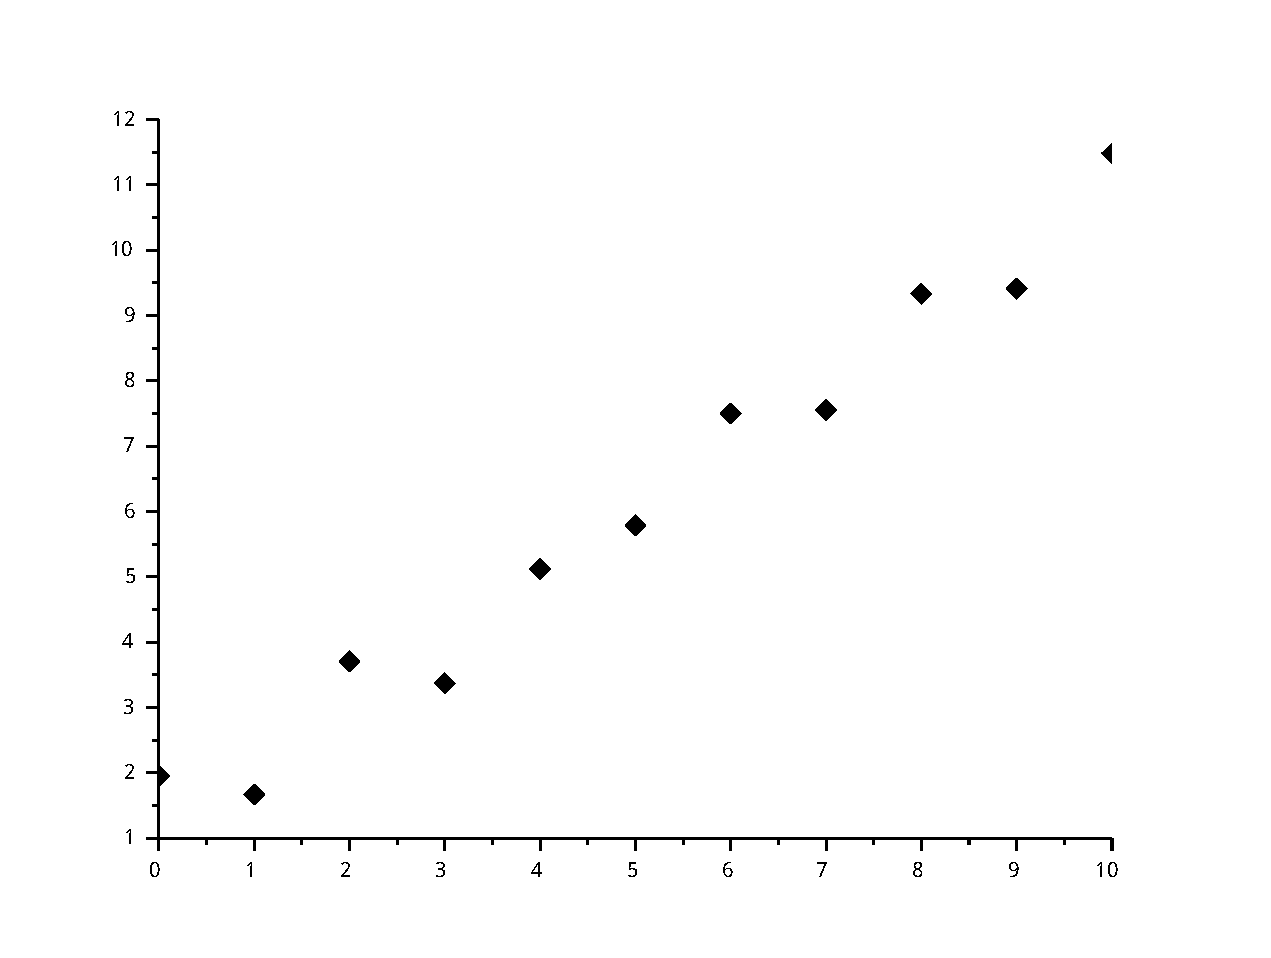
\includegraphics[scale=0.5]{./cap_derint/pics/graf_der}
\end{center}

Observe que as derivadas calculadas por diferenças finitas oscilam entre um valor pequeno e um grande em cada intervalo e além disso, a fórmula progressiva difere da regressiva significantemente. Por exemplo, por diferenças regressivas $f'(7)\approx \frac{(7,55 -  7,50)}{1}=0,05$ e por diferenças progressivas $f'(7)\approx \frac{(9,33 -  7,55)}{1}=1,78$. A melhor forma de calcular a derivada aqui é fazer um ajuste de curva. A reta que melhor ajusta os dados da tabela é $y=f(x)=1,2522727+0,9655455x$. Usando esse ajuste, temos $f'(7)\approx 0,9655455$.

\section*{Exercícios}

\begin{Exercise} Expanda a função suave $f(x)$ em um polinômio de Taylor adequado para obter as seguintes aproximações:
\begin{itemize}{\label{ex1}}
\item[a)] $f'(x)=\frac{f(x+h)-f(x)}{h}+O(h)$
\item[b)] $f'(x)=\frac{f(x)-f(x-h)}{h}+O(h)$
\item[c)] $f'(x)=\frac{f(x+h)-f(x-h)}{2h}+O(h^2)$
\item[d)] $f''(x)=\frac{f(x+h)-2f(x)+f(x-h)}{h^2}+O(h^2)$
\end{itemize}
\end{Exercise}

\begin{Exercise}
Use os esquemas numéricos do exercício \ref{ex1} para aproximar as seguintes derivadas:
\begin{itemize}
\item[a)] $f'(x)$ onde $f(x)=\sin(x)$ e $x=2$.
\item[b)] $f'(x)$ onde $f(x)=e^{-x}$ e $x=1$.
\item[c)] $f''(x)$ onde $f(x)=e^{-x}$ e $x=1$.
\end{itemize}

Use $h=10^{-2}$ e $h=10^{-3}$ e compare com os valores obtidos através da avaliação numérica das derivadas exatas.
\end{Exercise}

\begin{Exercise} Use a expansão da função $f(x)$ em torno de $x=0$ em polinômios de Taylor para encontrar os coeficientes $a_1$, $a_2$ e $a_3$ tais que
\begin{itemize}
\item[a)] $f'(0)=a_1f(0)+a_2f(h)+a_3f(2h) + O(h^2)$
\item[b)] $f'(0)=a_1f(0)+a_2f(-h)+a_3f(-2h) + O(h^2)$
\item[c)] $f'(0)=a_1f(-h_1)+a_2f(0)+a_3f(h_2) + O(h^2),~~|h_1|, |h_2|=O(h)$
\item[d)] $f''(0)=a_1f(0)+a_2f(h)+a_3f(2h) + O(h)$
\item[e)] $f''(0)=a_1f(0)+a_2f(-h)+a_3f(-2h) + O(h)$
\end{itemize}
\end{Exercise}
\begin{Answer}
\begin{itemize}
\item[a)] $f'(0)=\frac{-3f(0)+4f(h)-f(2h)}{2h} + O(h^2)$
\item[b)] $f'(0)=\frac{3f(0)-4f(-h)+f(-2h)}{2h} + O(h^2)$
\item[c)] $f'(0)=\frac{1}{h_1+h_2}l\left[-\frac{h_2}{h_1}f(-h_1) +\left(\frac{h_2}{h_1}-\frac{h_1}{h_2}\right)f(0)+ \frac{h_1}{h_2}f(h_2)\right]$
\item[d)] $f''(0)=\frac{f(0)-2f(h)+f(2h)}{h^2}+O(h)$
\item[e)] $f''(0)=\frac{f(0)-2f(-h)+f(-2h)}{h^2}+O(h)$
\end{itemize}
\end{Answer}

\begin{Exercise} As tensões  na entrada, $v_i$, e saída, $v_o$, de um amplificador foram medidas em regime estacionário conforme tabela abaixo.
$$\begin{array}{|c|c|c|c|c|c|c|c|c|c|c|}
\hline
    0. &   0.5  &   1.   &   1.5  &   2. &     2.5   &  3.  &    3.5  &   4.  &    4.5  &   5.\\
 \hline
 0.  &  1.05  &  1.83  &  2.69  &  3.83 &   4.56 &   5.49 &   6.56  &  6.11 &   7.06  &  8.29\\
 \hline
\end{array}
$$
onde  a primeira linha é a tensão de entrada em volts e a segunda linha é tensão de saída em volts.
Sabendo que o ganho é definido como $$\frac{\partial v_o}{\partial v_i}.$$ Calcule o ganho quando $v_i=1$ e $v_i=4.5$ usando as seguintes técnicas:
\begin{itemize}
\item[a)] Derivada primeira numérica de primeira ordem usando o próprio ponto e o próximo.
\item[b)] Derivada primeira numérica de primeira ordem usando o próprio ponto e o anterior.
\item[c)] Derivada primeira numérica de segunda ordem usando o ponto anterior e o próximo.
\item[d)] Derivada primeira analítica da função do tipo $v_0=a_1 v_i + a_3 v_i^3$ que melhor se ajusta aos pontos pelo critério dos mínimos quadrados.
\end{itemize}
$$\begin{array}{|c|c|c|c|c|}
\hline
 Caso &  a  &   b &   c   &   d \\
 \hline
 v_i=1 &    & ~\hspace{50pt}~  &   & ~\hspace{50pt}~ \\
 \hline
v_i=4.5 &~\hspace{50pt}~    &   &  ~\hspace{50pt}~   &\\
 \hline
\end{array}
$$
\ifisscilab
Dica:
\begin{verbatim}
y=[0 1.05 1.83 2.69 3.83 4.56 5.49 6.56 6.11 7.06 8.29]
\end{verbatim}
\fi
\end{Exercise}
\begin{Answer}
$$\begin{array}{|c|c|c|c|c|}
\hline
 Caso &  a  &   b &   c   &   d \\
 \hline
 v_i=1 & 1.72   & 1.56  &  1.64 & 1.86 \\
 \hline
v_i=4.5 &2.46    & 1.90  &  2.18  &1.14  \\
 \hline
\end{array}
$$
\end{Answer}


\section{Problemas de valor contorno}\index{problema de valor de contorno}

Nesta seção usaremos a aproximação numérica da derivada para resolver problemas de valor de contorno da forma
$$\left\{\begin{array}{l}-u_{xx}=f(x,u),~~ a<x<b.\\
u(a)=u_a\\
u(b)=u_b\end{array}
\right.
$$
Resolver numericamente o problema acima exige uma discretização do domínio $[a,b]$, ou seja, dividir o domínio em $N$ partes iguais, definindo
$$
h=\frac{b-a}{N}
$$
O conjunto de abcissas $x_i$, $i=1,...,N+1$ formam uma malha para o problema discreto. Nosso objetivo é encontrar as ordenadas $u_i=u(x_i)$ que satisfazem a versão discreta:
$$\left\{\begin{array}{l}-\frac{u_{i+1}-2u_i+u_{i-1}}{h^2}=f(x_i,u_i),~~ 2\leq i\leq N.\\
u_1=u_a\\
u_{N+1}=u_b\end{array}
\right.
$$
O vetor solução $(u_i)_{i=1}^{N+1}$ do problema é solução do sistema acima, que é linear se $f$ for linear em $u$ e não linear caso contrário.

\begin{ex}Encontre uma solução numérica para o problema de contorno:
$$\left\{\begin{array}{l}-u_{xx}+u=e^{-x},~~ 0<x<1.\\
u(0)=1\\
u(1)=2\end{array}
\right.
$$
\end{ex}
\begin{sol}
Observe que
$$
h=\frac{1}{N}
$$
e a versão discreta da equação é
$$\left\{\begin{array}{l}-\frac{u_{i+1}-2u_i+u_{i-1}}{h^2}+u_i=e^{-x_i},~~ 2\leq i\leq N.\\
u_1=1\\
u_{N+1}=2\end{array}
\right.
$$
ou seja,
$$\left\{\begin{array}{l}u_1=1\\-u_{i+1}+(2+h^2)u_i-u_{i-1}=h^2e^{-x_i},~~ 2\leq i\leq N.\\
u_{N+1}=2\end{array}
\right.
$$
que é um sistema linear. A sua forma matricial é:
$$
\left[\begin{array}{ccccccc}
1&0&0&\cdots&0&0&0\\
-1&2+h^2&-1&\cdots&0&0&0\\
0&-1&2+h^2&\cdots&0&0&0\\
\vdots&&&&\ddots&&\\
0&0&0&\cdots&-1&2+h^2&-1\\
0&0&0&\cdots&0&0&1\\
\end{array}\right]
\left[\begin{array}{c}u_1\\u_2\\u_3\\ \vdots\\ u_{N}\\u_{N+1}\end{array}\right]=
\left[\begin{array}{c}1\\h^2e^{-x_2}\\h^2e^{-x_3}\\ \vdots\\ h^2e^{-x_N}\\2\end{array}\right]
$$
Para $N=10$, temos a seguinte solução:
$$
\left[\begin{array}{c} 1,000000\\  1,0735083  \\1,1487032 \\ 1,2271979\\  1,3105564\\  1,4003172\\  1,4980159\\  1,6052067\\  1,7234836\\  1,8545022\\2,000000\end{array}\right]
$$  
\end{sol}

\section*{Exercícios}

\begin{Exercise}
 Considere o seguinte problema de valor de contorno para a equação de calor no estado estacionário:
$$\left\{\begin{array}{l}-u_{xx}=32,~~ 0<x<1.\\
u(0)=5\\
u(1)=10\end{array}
\right.
$$

Defina $u_j=u(x_j)$ onde $x_j={(j-1)}{h}$ e $j=1,\ldots,5$. Aproxime a derivada segunda por um esquema de segunda ordem e transforme a equação diferencial em um sistema de equações lineares. Escreva este sistema linear na forma matricial e resolva-o. Faça o mesmo com o dobro de subintervalos, isto é, com malha de 9 pontos. 
\end{Exercise}
\begin{Answer}
 

 $$\left[
  \begin{array}{ccccc}
         1 & 0& 0& 0& 0\\
         -1 & 2 & -1 &0&0\\
         0&-1 & 2 & -1 &0\\
         0&0&-1 & 2 & -1 \\
         0 & 0& 0& 0& 1\\
        \end{array}
\right]
\left[
  \begin{array}{c}
     u_1\\ u_2\\u_3\\u_4 \\ u_5
   \end{array}
\right]
=
\left[
  \begin{array}{c}
     5\\ 2\\2\\2 \\ 10
   \end{array}
\right]
$$


Solução:  [5, 9.25, 11.5, 11.75, 10]    

$$\left[
  \begin{array}{ccccccccc}
         1 & 0& 0& 0& 0& 0& 0& 0& 0\\
         -1 & 2 & -1 &0&0& 0& 0& 0& 0\\
         0&-1 & 2 & -1 &0& 0& 0& 0& 0\\
         0&0&-1 & 2 & -1 & 0& 0& 0& 0\\
         0&0&0&-1 & 2 & -1 & 0& 0& 0\\
         0&0&0&0&-1 & 2 & -1 & 0& 0\\
         0&0&0&0&0&-1 & 2 & -1 & 0\\
         0&0&0&0&0&0&-1 & 2 & -1\\
         0 & 0& 0& 0& 0& 0& 0& 0& 1\\
        \end{array}
\right]
\left[
  \begin{array}{c}
     u_1\\ u_2\\u_3\\u_4 \\u_5\\ u_6\\u_7\\u_8\\u_9
   \end{array}
\right]
=
\left[
  \begin{array}{c}
     5\\ 0.5\\0.5\\0.5\\ 0.5\\0.5\\0.5\\0.5 \\ 10
   \end{array}
\right]
$$

Solução:  [5, 7.375, 9.25, 10.625, 11.5, 11.875, 11.75, 1.125, 10]    
\end{Answer}


\begin{Exercise} Considere o seguinte problema de valor de contorno para a equação de calor no estado estacionário:
$$\left\{\begin{array}{l}-u_{xx}=200e^{-(x-1)^2},~~ 0<x<2.\\
u(0)=120\\
u(2)=100\end{array}
\right.
$$
Defina $u_j=u(x_j)$ onde $x_j={(j-1)}{h}$ e $j=1,\ldots,21$. Aproxime a derivada segunda por um esquema de segunda ordem e transforme a equação diferencial em um sistema de equações lineares. Resolva o sistema linear obtido.


\end{Exercise}
\begin{Answer}
120.    133.56    146.22    157.83    168.22    177.21    184.65    190.38    194.28    196.26    196.26    194.26    190.28    184.38    176.65    167.21  156.22    143.83    130.22    115.56    100.
\end{Answer}



\begin{Exercise} Considere o seguinte problema de valor de contorno para a equação de calor no estado estacionário:
$$\left\{\begin{array}{l}-u_{xx}=200e^{-(x-1)^2},~~ 0<x<2.\\
u'(0)=0\\
u(2)=100\end{array}
\right.
$$
Defina $u_j=u(x_j)$ onde $x_j={(j-1)}{h}$ e $j=1,\ldots,21$. Aproxime a derivada segunda por um esquema de segunda ordem, a derivada primeira na fronteira por um esquema de primeira ordem e transforme a equação diferencial em um sistema de equações lineares. Resolva o sistema linear obtido.
\end{Exercise}

\begin{Answer}
391.13    391.13    390.24    388.29    385.12    380.56    374.44    366.61    356.95    345.38    331.82    316.27    298.73    279.27    257.99    234.99    210.45    184.5    157.34    129.11    100.
\end{Answer}


\begin{Exercise} Considere o seguinte problema de valor de contorno para a equação de calor no estado estacionário com um termo não-linear de radiação:
$$\left\{\begin{array}{l}-u_{xx}=100- \frac{u^4}{10000},~~ 0<x<2.\\
u(0)=0\\
u(2)=10\end{array}
\right.
$$
Defina $u_j=u(x_j)$ onde $x_j={(j-1)}{h}$ e $j=1,\ldots,21$. Aproxime a derivada segunda por um esquema de segunda ordem e transforme a equação diferencial em um sistema de equações não lineares. Resolva o sistema  obtido. Expresse  a solução com dois algarismos depois do separador decimal. Dica: Veja problema 38 da lista 2, seção de sistemas não lineares.
\end{Exercise}

\begin{Answer}
0.,    6.57,    12.14,    16.73,    20.4,    23.24,    25.38,    26.93 ,   28,    28.7,    29.06,    29.15,    28.95,    28.46, 27.62 ,   26.36,    24.59,    22.18,    19.02,    14.98,    10.
\end{Answer}


\begin{Exercise} Considere o seguinte problema de valor de contorno para a equação de calor no estado estacionário com um termo não-linear de radiação e um termo de convecção:
$$\left\{\begin{array}{l}-u_{xx}+3u_x=100- \frac{u^4}{10000},~~ 0<x<2.\\
u'(0)=0\\
u(2)=10\end{array}
\right.
$$
Defina $u_j=u(x_j)$ onde $x_j={(j-1)}{h}$ e $j=1,\ldots,21$. Aproxime a derivada segunda por um esquema de segunda ordem, a derivada primeira na fronteira por um esquema de primeira ordem, a derivada primeira no interior por um esquema de segunda ordem e transforme a equação diferencial em um sistema de equações não lineares. Resolva o sistema  obtido.
\end{Exercise}
\begin{Answer}
u(0)=31.62, u(1)=31.50, u(1.9)=18.17
\end{Answer}

\begin{Exercise} Considere o seguinte problema de valor de contorno:
$$\left\{\begin{array}{l}-u''+2u'=e^{-x}- \frac{u^2}{100},~~ 1<x<4.\\
u'(1)+u(1)=2\\
u'(4)=-1\end{array}
\right.
$$
Defina $u_j=u(x_j)$ onde $x_j=1+{(j-1)}{h}$ e $j=1,\ldots,101$. Aproxime a derivada segunda por um esquema de segunda ordem, a derivada primeira na fronteira por um esquema de primeira ordem, a derivada primeira no interior por um esquema de segunda ordem e transforme a equação diferencial em um sistema de equações não lineares. Resolva o sistema  obtido.
\end{Exercise}
\begin{Answer}
u(1)=1.900362, u(2.5)=1.943681, u(4)=1.456517
\end{Answer}

\section{Integração numérica}\index{integração numérica}

Considere o problema de calcular a área entre uma função positiva, o eixo $x$ e as retas $x=a$ e $x=b$. O valor exato dessa área é calculada fazendo uma aproximação por retângulos com bases iguais e depois tomando o limite quando o número de retângulos tende ao infinito:
$$
A=\lim_{n\to\infty}\sum_{i=1}^nf(x_i)h_n,
$$
onde $h_n=\frac{b-a}{n}$ é o tamanho da base dos retângulo e $f(x_i)$, $1\leq i\leq n$, $a+(i-1)h\leq x_i\leq a+ih$, é a altura dos retângulos. Essa definição é generalizada para cálculo de integrais num intervalo $[a,b]$:
$$
\int_a^bf(x)dx=\lim_{n\to\infty}\sum_{i=1}^nf(x_i)h_n.
$$
A figura abaixo mostra um exemplo quando $f(x)=x^2+1$, $0\leq x\leq 2$. Temos a aproximação por um retângulo com base $h_1=2$, depois com dois retângulos de base $h_2=1$ e, finalmente com quatro retângulo de bases $h_3=0,5$.
\begin{center}
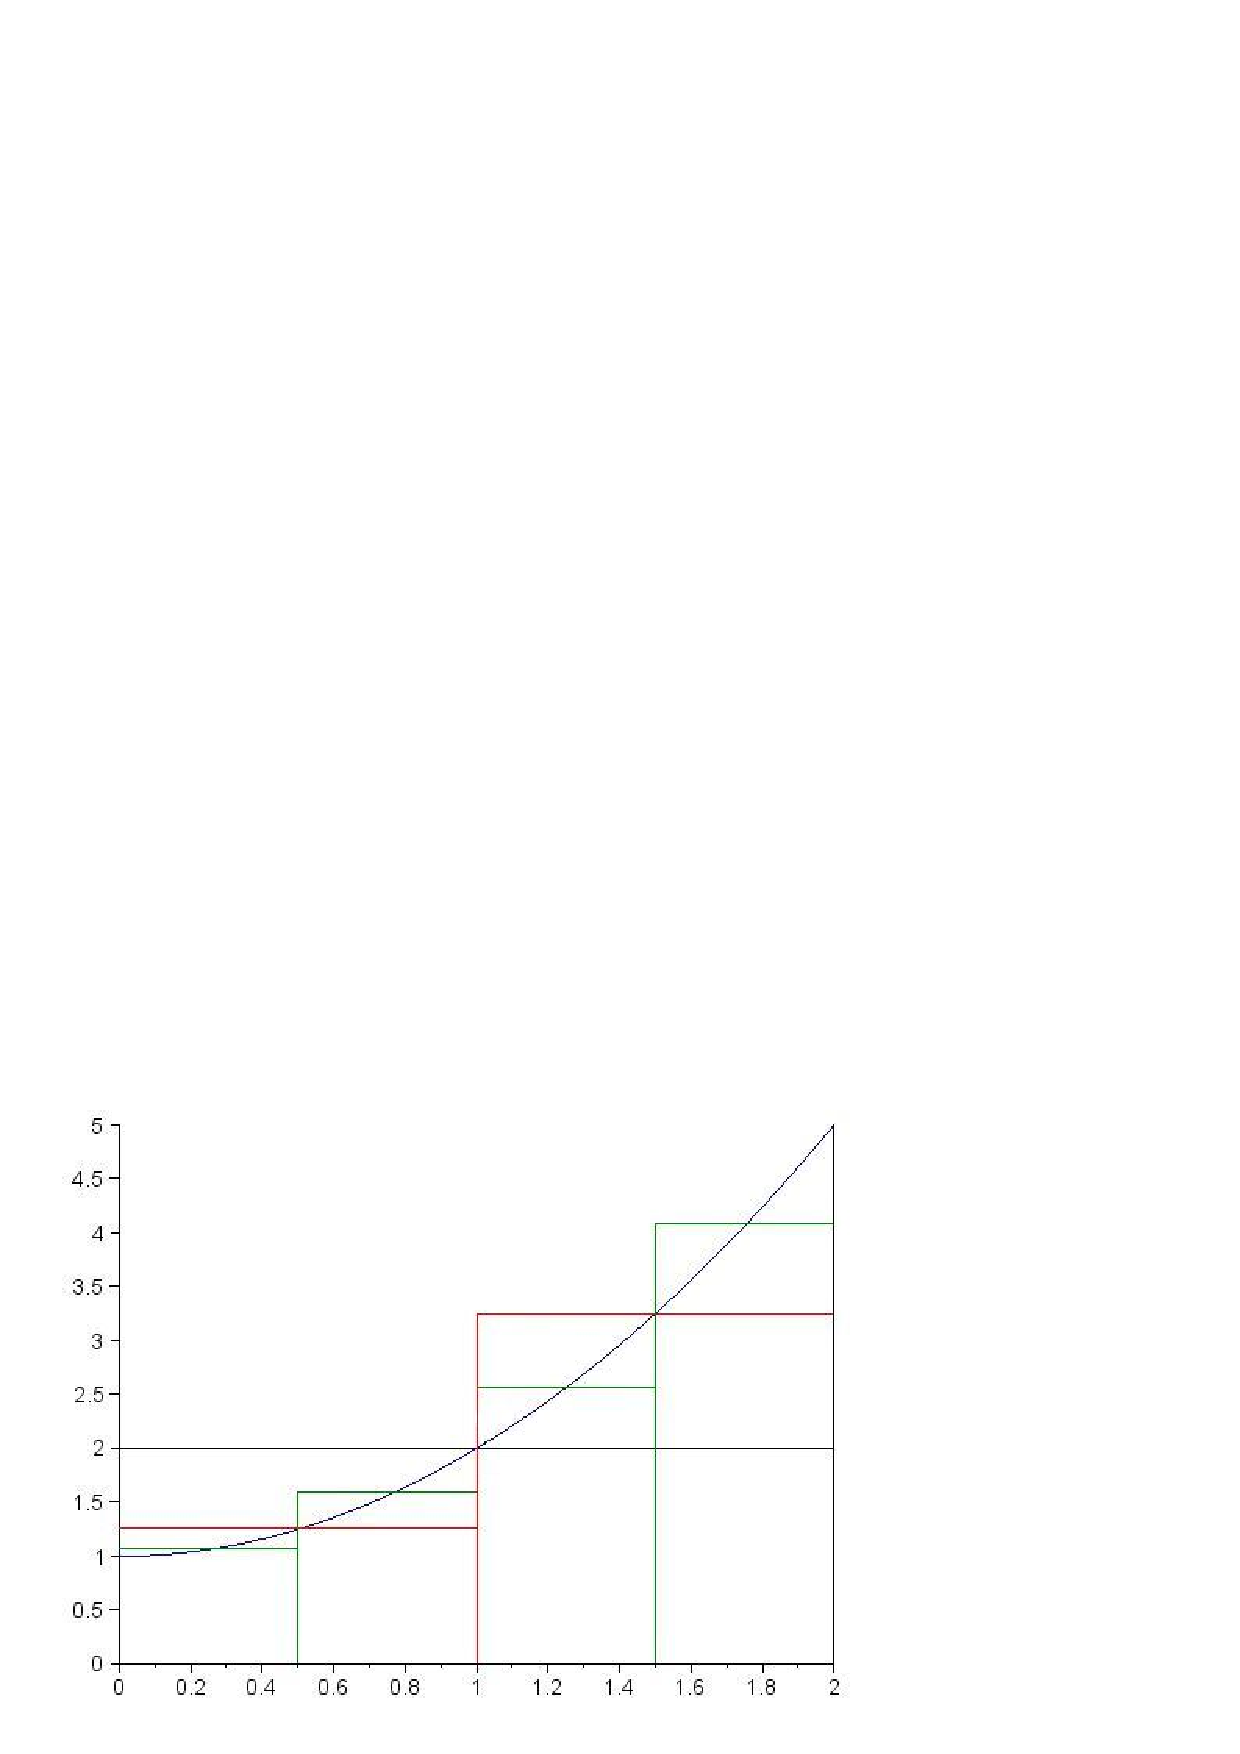
\includegraphics[scale=0.7]{./cap_derint/pics/int_1}
\end{center}

Os valores aproximados para a integral são dados na tabela:
$$
\begin{array}{|c|c|c|c|c|}
\hline
&h_1=2&h_2=1&h_3=0,5&h_4=0,25\\
\hline
\int_0^2(x^2+1)dx&h_1f(1)=4&h_2f(0,5)+h_2f(1,5)=4,5&4,625&4,65625\\
\hline
\end{array}
$$
Observe que
$$
\int_0^2(x^2+1)dx=\left[\frac{x^3}{3}+x\right]_0^2=\frac{8}{3}+2=4,6666667
$$

\subsection{Regras de Newton-Cotes}\index{integração numérica!regras de Newton-Cotes}

A integral de uma função num intervalo $[a,b]$, também chamada de quadratura numérica, é aproximada pela soma
$$
\int_a^bf(x)dx\approx\sum_{i=1}^na_if(x_i),
$$
onde $x_i$, $1\leq i\leq n$, são pontos distintos do intervalo $[a,b]$. Nessa definição, a integral $\int_0^2(x^2+1)dx$ (dada na seção \ref{sec_int}) usando uma aproximação por retângulo usa apenas um ponto, o ponto médio do intervalo ($x_1=1$), e a soma se reduz a uma parcela ($(2-0)f(1)$). A fórmula geral para essa caso, chamado de regra do ponto médio é:
\begin{equation}{\label{ponto_médio_1}}
\int_a^bf(x)dx\approx (b-a)f\left(\frac{a+b}{2}\right):=hf(x_1).
\end{equation}

\subsubsection{Regra do ponto médio}\index{integração numérica!regra do ponto médio}
A regra do ponto médio (\ref{ponto_médio_1}) pode ser deduzida mais formalmente usando a expansão de Taylor
$$
f(x)=f(x_1)+f'(x_1)(x-x_1)+\frac{f''(\xi(x))}{2}(x-x_1)^2
$$
que leva a integral
$$
\int_a^b f(x)dx=\int_a^b f(x_1) dx+f'(x_1)\int_a^b(x-x_1)dx +\int_a^b\frac{f''(\xi(x))}{2}(x-x_1)^2dx.
$$
Usando o teorema do valor médio para integrais e que $h=b-a$ e $x_1=(a+b)/2$, temos:
\begin{align*}
\int_a^b f(x)dx &= h f(x_1) + f'(x_1)\int_a^b(x-x_1)dx+f''(\eta)\int_a^b\frac{1}{2}(x-x_1)^2dx\\
&= h f(x_1) +f'(x_1)\left[\frac{(x-x_1)^2}{2}\right]_a^b+f''(\eta)\left[\frac{1}{6}(x-x_1)^3\right]_a^b\\
&= h f(x_1) +f'(x_1)\left[\frac{(b-x_1)^2}{2}-\frac{(a-x_1)^2}{2}\right]\\
&+f''(\eta)\left[\frac{1}{6}(b-x_1)^3-\frac{1}{6}(a-x_1)^3\right]\\
&= h f(x_1) +\frac{h^3f''(\eta)}{3}.
\end{align*}
para $a\leq \eta\leq b$.

\begin{ex}
Use a regra do ponto médio para aproximar a integral
$$
\int_0^1e^{-x^2}dx.
$$
Depois divida a integral em duas
$$
\int_0^{1/2}e^{-x^2}dx+\int_{1/2}^{1}e^{-x^2}dx.
$$
e aplique a regra do ponto médio em cada uma delas. Finalmente, repita o processo dividindo em quatro integrais.

Usando o intervalo $[0,1]$, temos $h=1$ e $x_1=1/2$. A regra do ponto médio resulta em
$$
\int_0^1e^{-x^2}dx\approx 1\cdot e^{-1/4}=0,7788008
$$
Usando dois intervalos, $[0,1/2]$ e $[1/2,1]$ e usando a regra do ponto médio em cada um dos intervalos, temos:
$$
\int_0^1e^{-x^2}dx\approx 0,5\cdot e^{-1/16}+0,5\cdot e^{-9/16})=0,4697065+0,2848914=0,7545979
$$
Agora, usando quatro intervalos, temos
$$
\int_0^1e^{-x^2}dx\approx 0,25\cdot e^{-1/64}+0,25\cdot e^{-9/64}+0,25\cdot e^{-25/64}+0,25\cdot e^{-49/64}=0,7487471
$$
Observe que o valor da integral é
$$
\int_0^1e^{-x^2}dx=0,7468241330.
$$
\end{ex}


A forma natural de obter as regras de integração é usar o polinômio de Lagrange que passa pelo pontos $\{(x_i,f(x_i))\}_{i=1}^n$
$$
f(x)=P_n(x)+\text{termo de erro}=\sum_{i=1}^nf(x_i)L_i(x) +\prod_{i=1}^n(x-x_i)\frac{f^{(n+1)}(\xi(x))}{(n+1)!}.
$$
e integramos
$$
\int_a^bf(x)dx=\sum_{i=1}^n\left[f(x_i)\int_a^bL_i(x)dx\right] +\frac{1}{(n+1)!}\int_a^b\prod_{i=1}^n(x-x_i)f^{(n+1)}(\xi(x))dx.
$$
A fórmula de quadratura então é
$$
\int_a^bf(x)dx\approx\sum_{i=1}^na_if(x_i),
$$
onde
$$
a_i=\int_a^bL_i(x)dx
$$

\subsubsection{Regra do Trapézio}\index{integração numérica!regra do trapézio}

A regra do trapézio consiste em aproximar a integral por um trapézio em vez de um retângulo, como fizemos. Para isso, o polinômio de Lagrange deve ser uma reta, como mostra a figura.
\begin{center}
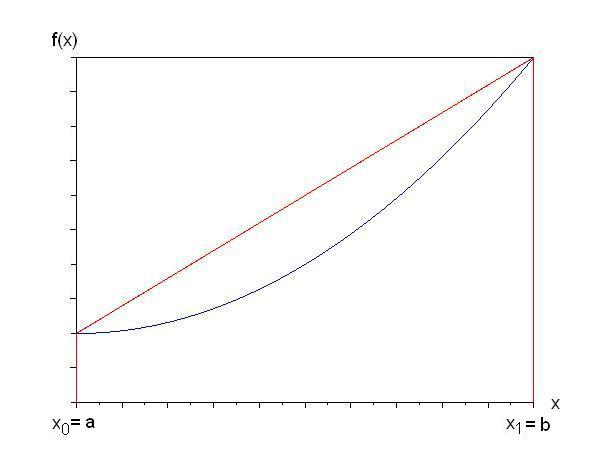
\includegraphics[scale=0.7]{./cap_derint/pics/int_2}
\end{center}

O polinômio de Lagrange de primeira ordem que passa por $(x_0,f(x_0)):=(a,f(a))$ e $(x_1,f(x_1)):=(b,f(b))$ é dado por
$$
P_1(x)=f(x_0)\frac{(x-x_0)}{(x_1-x_0)}+f(x_1)\frac{(x-x_1)}{(x_0-x_1)}=f(x_0)\frac{(x-x_0)}{h}-f(x_1)\frac{(x-x_1)}{h},
$$
onde $h=x_1-x_0$. Podemos integrar a função $f(x)$ aproximando-a por esse polinômio:
\begin{equation*}
  \begin{split}
    \int_a^bf(x)dx &= f(x_0)\int_a^b\frac{(x-x_0)}{h}dx-f(x_1)\int_a^b\frac{(x-x_1)}{h}dx\\
    &+\frac{1}{2!}\int_a^b(x-x_0)(x-x_1)f''(\xi(x))dx.   
  \end{split}
\end{equation*}
Pelo teorema do valor médio, existe $a\leq \eta\leq b$ tal que $\int_a^bf(\xi(x))g(x)dx=f(\eta)\int_a^bg(x)dx$ e, portanto,
\begin{equation*}
  \begin{split}
    \int_a^bf(x)dx&= f(x_0)\left[\frac{(x-x_0)^2}{2h}\right]_{x_0}^{x_1}-f(x_1)\left[\frac{(x-x_1)^2}{2h}\right]_{x_0}^{x_1}\\
    &+ \frac{f''(\eta)}{2}\left[\frac{x^3}{3}-\frac{x^2}{2}(x_1+x_0)+x_0x_1x\right]_{x_0}^{x_1}\\
&= f(x_0)\frac{(x_1-x_0)^2}{2h}+f(x_1)\frac{(x_0-x_1)^2}{2h}\\
&+ \frac{f''(\eta)}{2}\left(\frac{x_1^3}{3}-\frac{x_1^2}{2}(x_1+x_0)+x_0x_1x_1-\frac{x_0^3}{3}+\frac{x_0^2}{2}(x_1+x_0)-x_0x_1x_0\right)\\
&= f(x_0)\frac{h^2}{2h}+f(x_1)\frac{h^2}{2h}\\
&+ \frac{f''(\eta)}{2}\frac{2x_1^3-3x_1^2(x_1+x_0)+6x_1^2x_0-2x_0^3+3x_0^2(x_1+x_0)-6x_1x_0^2}{6}\\
&= \frac{h}{2}(f(x_0)+f(x_1))+\frac{f''(\eta)}{12}\left(x_0^3-3x_0^2x_1+3x_1^2x_0-x_1^3\right)\\
&= \frac{h}{2}(f(x_0)+f(x_1))-\frac{h^3f''(\eta)}{12}    
  \end{split}
\end{equation*}

\begin{ex}
Use a regra do trapézio para aproximar a integral
$$
\int_0^1e^{-x^2}dx.
$$
Depois divida a integral em duas
$$
\int_0^{1/2}e^{-x^2}dx+\int_{1/2}^{1}e^{-x^2}dx.
$$
e aplica a regra do trapézio em cada uma delas. Finalmente, repita o processo dividindo em quatro integrais.
\end{ex}
Usando o intervalo $[0,1]$, temos $h=1$, $x_0=0$ e $x_1=1$. A regra do trapézio resulta em
$$
\int_0^1e^{-x^2}dx\approx \frac{1}{2}(e^{0}+e^{-1})=0,6839397
$$
Usando dois intervalos, $[0,1/2]$ e $[1/2,1]$ e usando a regra do trapézio em cada um dos intervalos, temos:
\begin{align*}
\int_0^1e^{-x^2}dx &\approx \frac{0,5}{2}\left(e^{0}+e^{-1/4}\right) + \frac{0,5}{2}\left(e^{-1/4}+e^{-1}\right) \\
&= 0,4447002+0,2866701 =0,7313703.
\end{align*}
Agora, usando quatro intervalos, temos
\begin{align*}
\int_0^1e^{-x^2}dx &\approx \frac{0,25}{2}\left(e^{0}+e^{-1/16}\right) + \frac{0,25}{2}\left(e^{-1/16}+e^{-1/4}\right) \\
&+ \frac{0,25}{2}\left(e^{-1/4}+e^{-9/16}\right)+\frac{0,25}{2}\left(e^{-9/16}+e^{-1}\right) \\
&= 0,7429841
\end{align*}

\subsubsection{Regra de Simpson}\index{integração numérica!regra de Simpson}
A regra de Simpson consiste em aproximar a integral usando três pontos do intervalo:
$$
x_0=a,\qquad x_1:=\frac{a+b}{2}=x_0+h \qquad \text{e}\qquad x_2:=b=x_1+h.
$$
com $h = (b-a)/2$. Para isso, o polinômio de Lagrange deve ser uma parábola:
\begin{equation*}
  \begin{split}
    P_2(x) &= f(x_0)\frac{(x-x_1)(x-x_2)}{(x_0-x_1)(x_0-x_2)} + f(x_1)\frac{(x-x_0)(x-x_2)}{(x_1-x_0)(x_1-x_2)}\\
    &+ f(x_2)\frac{(x-x_0)(x-x_1)}{(x_2-x_0)(x_2-x_1)}.
  \end{split}
\end{equation*}
Se usarmos o mesma metodologia da regra dos trapézios, calcularemos
$$
\int_a^bf(x)dx=\int_a^bP_2(x)dx+\int_a^b\frac{(x-x_0)(x-x_1)(x-x_2)}{6}f'''(\xi(x))dx
$$
e obteremos o fórmula de Simpson com um erro de quarta ordem. O fato é que a regra de Simpson tem ordem cinco e, para isso, usaremos uma abordagem alternativa. Considere o polinômio de Taylor
$$
f(x)=f(x_1)+f'(x_1)(x-x_1)+\frac{f''(x_1)}{2}(x-x_1)^2+\frac{f'''(x_1)}{6}(x-x_1)^3+\frac{f^{(4)}(\xi(x))}{24}(x-x_1)^4,
$$
onde $x_0\leq\xi(x)\leq x_2$ e integre no intervalo $[a,b]=[x_0,x_2]$:
\begin{equation*}
  \begin{split}
    \int_a^bf(x)dx&= \left[f(x_1)(x-x_1)+f'(x_1)\frac{(x-x_1)^2}{2} + \frac{f''(x_1)}{6}(x-x_1)^3\right. \\
      &\left. + \frac{f'''(x_1)}{24}(x-x_1)^4\right]_{x_0}^{x_2}\\
      &+ \frac{1}{24}\int_{x_0}^{x_2}f^{(4)}(\xi(x))(x-x_1)^4dx,    
  \end{split}
\end{equation*}
Pelo teorema do valor médio, existe $x_0\leq\eta\leq x_2$ tal que
\begin{equation*}
  \begin{split}
    \int_a^bf(x)dx&= \left[f(x_1)(x-x_1)+f'(x_1)\frac{(x-x_1)^2}{2}+\frac{f''(x_1)}{6}(x-x_1)^3\right.\\
    &+\left.\frac{f'''(x_1)}{24}(x-x_1)^4\right]_{x_0}^{x_2}\\
    &+ \frac{f^{(4)}(\eta)}{24}\int_{x_0}^{x_2}(x-x_1)^4dx\\
    &= \left[f(x_1)(x-x_1)+f'(x_1)\frac{(x-x_1)^2}{2}+\frac{f''(x_1)}{6}(x-x_1)^3\right.\\
    &+\left.\frac{f'''(x_1)}{24}(x-x_1)^4\right]_{x_0}^{x_2}\\
    &+ \frac{f^{(4)}(\eta)}{120}\left[(x-x_1)^5\right]_{x_0}^{x_2}    
  \end{split}
\end{equation*}
Usando o fato que
$$
(x_2-x_1)^3-(x_0-x_1)^3=2h^3,
$$
$$
(x_2-x_1)^4-(x_0-x_1)^4=0
$$
e
$$
(x_2-x_1)^5-(x_0-x_1)^5=2h^5,
$$
temos
$$
\int_a^bf(x)dx=2hf(x_1)+\frac{h^3}{3}f''(x_1)+\frac{h^5f^{(4)}(\eta)}{60}.
$$
Usando a diferenças finitas centrais para a derivada segunda:
$$
f''(x_1)=\frac{f(x_0)-2f(x_1)+f(x_2)}{h^2}+\frac{h^2}{12}f^{(4)}(\eta_1),
$$
$x_0\leq \eta_1\leq x_2$, temos
\begin{eqnarray*}
\int_a^bf(x)dx&=&2hf(x_1)+\frac{h^3}{3}\left(\frac{f(x_0)-2f(x_1)+f(x_2)}{h^2}+\frac{h^2}{12}f^{(4)}(\eta_1)\right)\\
&+&\frac{h^5f^{(4)}(\eta)}{60}\\
&=&\frac{h}{3}\left(f(x_0)+4f(x_1)+f(x_2)\right)-\frac{h^5}{12}\left(\frac{1}{3}f^{(4)}(\eta_1)-\frac{1}{5}f^{(4)}(\eta)\right).
\end{eqnarray*}
Pode-se mostrar que é possível escolher $\eta_2$ que substitua $\eta$ e $\eta_1$ com a seguinte estimativa
$$
\int_a^bf(x)dx=\frac{h}{3}\left(f(x_0)+4f(x_1)+f(x_2)\right)-\frac{h^5}{90}f^{(4)}(\eta_2).
$$

\begin{ex}
Use a regra de Simpson para aproximar a integral
$$
\int_0^1e^{-x^2}dx.
$$
Depois divida a integral em duas
$$
\int_0^{1/2}e^{-x^2}dx+\int_{1/2}^{1}e^{-x^2}dx.
$$
e aplica a regra de Simpson em cada uma delas.
\end{ex}
Usando o intervalo $[0,1]$, temos $h=1/2$, $x_0=0$, $x_1=1/2$ e $x_2=1$. A regra de Simpson resulta em
$$
\int_0^1e^{-x^2}dx\approx \frac{0,5}{3}(e^{0}+4e^{-1/4}+e^{-1})=0,7471804
$$
Usando dois intervalos, $[0,1/2]$ e $[1/2,1]$ e usando a regra do trapézio em cada um dos intervalos, temos:
$$
\int_0^1e^{-x^2}dx\approx \frac{0,25}{3}(e^{0}+4e^{-1/16}+e^{-1/4})+\frac{0,25}{3}(e^{-1/4}+4e^{-9/16}+e^{-1})=0,7468554
$$

\subsection{Regras compostas}\index{integração numérica!regras compostas}

Vimos que em todas as estimativas de erro que derivamos, o erro depende do tamanho do intervalo de integração. Uma estratégia para reduzir o erro consiste em particionar o intervalo de integração em diversos subintervalos menores:
\begin{equation*}
\int_{a}^b f(x)dx=\sum_{i=1}^{n} \int_{x_i}^{x_{i+1}} f(x)dx  
\end{equation*}
onde $x_i = a + (i-1)h$, $h = (b-a)/n$ e $i = 1,2,\dotsc,n+1$, sendo $n$ o número de subintervalos da partição do intervalo de integração. Depois, aplica-se um método simples de integração em cada subintervalo.

\subsubsection{Método composto dos trapézios}\index{integração numérica!método composto!dos trapézios}
A \emph{regra composta dos trapézios} assume a seguinte forma:
\begin{align*}
  \int_{a}^b f(x)dx &= \sum_{i=1}^{n} \int_{x_i}^{x_{i+1}}f(x)\,dx \\
  &\approx \sum_{i=1}^{n} \frac{x_{i+1}-x_i}{2}\left[f(x_i)+f(x_{i+1})\right]
\end{align*}
Como $h = x_{i+1} - x_i$, temos:
\begin{align*}
\int_{a}^b f(x)\,dx &\approx \frac{h}{2}\sum_{k=1}^{N_i}\left[f(x_k)+f(x_{k+1})\right]\\
& = \frac{h}{2}\left[f(x_1)+2f(x_2)+2f(x_3)+\cdots + 2f(x_{N_i})+f(x_{N_i+1})\right]\\
& = \frac{h}{2}\left[f(x_1) + f(x_{N_i+1})\right] + h\sum_{i=2}^{N_i} f(x_i)
\end{align*}

\ifisscilab
\subsubsection{Código Scilab: Trapézio Composto}
O código Scilab abaixo é uma implementação do método do trapézio composto para calcular:
\begin{equation*}
  \int_a^b f(x)\,dx = \frac{h}{2}\left[f(x_1) + f(x_{n+1})\right] + h\sum_{i=2}^n f(x_i) + O(h^3),
\end{equation*}
onde $h = (b-a)/n$ e $x_i = a + (i-1)h$, $i=1,2,\dotsc,n+1$. Os parâmetros de entrada são: \verb+f+ o integrando definido como uma função no Scilab, \verb+a+ o limite inferior de integração, \verb+b+ o limite superior de integração, \verb+n+ o número de subintervalos desejado. A variável de saída é \verb+y+ e corresponde a aproximação calculada de $\int_a^b f(x)\, dx$.

\verbatiminput{./cap_derint/codes/trap_comp/trap_comp.sci}
\fi

\subsubsection{Método composto de Simpson}\index{integração numérica!método composto!de Simpson}
Já a regra composta de Simpson assume a seguinte forma:
\begin{align*}
  \int_{a}^b f(x)\,dx &= \sum_{k=1}^{n} \int_{x_k}^{x_{k+1}} f(x)dx \\
  &\approx \sum_{k=1}^{n} \frac{x_{x+1}-x_k}{6}\left[f(x_k) + 4f\left(\frac{x_{k+1}+x_k}{2}\right)+f(x_{k+1})\right]
\end{align*}
onde, como anteriormente, $x_k = a + (k-1)h$, $h = (b-a)/n$ e $i = 1,2,\dotsc,n+1$, sendo $n$ o número de subintervalos da partição do intervalo de integração. Podemos simplificar o somatório acima, escrevendo:
\begin{equation*}
  \int_{a}^b f(x)\,dx \approx \frac{h}{3}\left[f(x_1) + 2\sum_{i=1}^{n-1} f(x_{2i+1}) + 4\sum_{i=1}^{n} f(x_{2i}) + f(x_{2n+1})\right] + O(h^5)
\end{equation*}
onde, agora, $h = (b-a)/(2n)$, $x_i = a + (i-1)h$, $i=1,2,\dotsc,2n+1$.

\ifisscilab
\subsubsection{Código Scilab: Simpson Composto}
O código Scilab abaixo é uma implementação do método de Simpson composto para calcular:
\begin{equation*}
  \int_a^b f(x)\,dx = \frac{h}{3}\left[f(x_1) + 2\sum_{i=1}^{n-1} f(x_{2i+1}) + 4\sum_{i=1}^{n} f(x_{2i}) + f(x_{2n+1})\right] + O(h^3),
\end{equation*}
onde $h = (b-a)/(2n)$ e $x_i = a + (i-1)h$, $i=1,2,\dotsc,2n+1$. Os parâmetros de entrada são: \verb+f+ o integrando definido como uma função no Scilab, \verb+a+ o limite inferior de integração, \verb+b+ o limite superior de integração, \verb+n+ o número de subintervalos desejado. A variável de saída é \verb+y+ e corresponde a aproximação calculada de $\int_a^b f(x)\, dx$.
\verbatiminput{./rotinas/Derivacao_e_integracao/simp_comp.sci}
\fi

\begin{ex}Calcule numericamente a integral
$$
\int_0^2 x^2 e^{x^2}dx
$$
pelas regras compostas do ponto médio, trapézio e Simpson variando o número de intervalos \\$N_i=1,\ 2,\ 3,\ 6,\ 12,\ 24,\ 48,\ 96$.
\end{ex}
\begin{equation*}
\begin{array}{|c|c|c|c|}
\hline
n&\hbox{ponto médio}&\hbox{Trapézios}&\hbox{Simpson}\\\hline
1&5,4365637&218,3926&76,421909\\\hline
2&21,668412&111,91458&51,750469\\\hline
3&31,678746&80,272022&47,876505\\\hline
6&41,755985&55,975384&46,495785\\\hline
12&45,137529&48,865685&46,380248\\\hline
24&46,057757&47,001607&46,372373\\\hline
48&46,292964&46,529682&46,37187\\\hline
96&46,352096&46,411323&46,371838\\
\hline
\end{array}  
\end{equation*}

\subsection{O método de Romberg}\index{integração numérica!método de Romberg}
O método de Romberg é um método simplificado para construir quadraturas de alta ordem.

Considere o método de trapézios composto aplicado à integral
$$\int_a^bf(x)dx$$
Defina $I(h)$ a aproximação desta integral pelo método dos trapézios composto com  malha de largura constante igual a h. Aqui $h=\frac{b-a}{N_i}$ para algum $N_i$ inteiro, i.e.:
$$I(h)=\frac{h}{2}\left[f(a)+2\sum_{j=2}^{N_i} f(x_j)+ f(b)\right],~~~N_i=\frac{b-a}{h}$$

\begin{teo} Se $f(x)$ é uma função analítica no intervalo $(a,b)$, então a função $I(h)$ admite uma representação na forma
$$I(h)=I_0 + I_2 h^2 + I_4{h^4}+ I_6{h^6}+\ldots$$
\end{teo}
Para um demonstração, veja \cite{DEMAILLY}. Em especial observamos que
$$\int_a^b f(x)dx = \lim_{h\to 0}I(h)=I_0$$
Ou seja, o valor exato da integral procurada é dado pelo coeficiente $I_0$.

A ideia central do método de Romberg, agora, consiste em usar a extrapolação de Richardson para construir métodos de maior ordem a partir do métodos dos trapézios para o intervalo $(a,b)$
\begin{ex} \label{exemplo_romberg_1}Construção do método de quarta ordem.
\begin{eqnarray*}
I(h)&=&I_0 + I_2 h^2 + I_4{h^4}+ I_6{h^6}+\ldots\\~\\
I\left(\frac{h}{2}\right)&=&I_0 + I_2 \frac{h^2}{4} + I_4\frac{h^4}{16}+ I_6\frac{h^6}{64}+\ldots\\
\end{eqnarray*}
Usamos agora uma eliminação gaussiana para obter o termo $I_0$:
\begin{eqnarray*}
\frac{4I(h/2)-I(h)}{3}=I_0-\frac{1}{4}I_4h^4-\frac{5}{16}I_6h^6+\ldots
\end{eqnarray*}
Vamos agora aplicar a fórmula para $h=b-a$,
\begin{eqnarray*}
I(h)&=& \frac{h}{2} \left[f(a)+f(b)\right]\\
I(h/2)&=& \frac{h}{4} \left[f(a)+2f\left(c\right)+f(b)\right],~~ c=\frac{a+b}{2}\\
\end{eqnarray*}

\begin{eqnarray*}
\frac{4I(h/2)-I(h)}{3}&=&\frac{h}{3}\left[f(a)+2f\left(c\right)+f(b)\right]-\frac{h}{6} \left[f(a)+f(b)\right]\\
&=&\frac{h}{6}\left[f(a)+4f\left(c\right)+f(b)\right]
\end{eqnarray*}
Observe que esquema coincide com o método de Simpson.
\end{ex}

A partir de agora, usaremos a seguinte notação
\begin{eqnarray*}
R_{1,1}&=&I(h)\\
R_{2,1}&=&I(h/2)\\
R_{3,1}&=&I(h/4)\\
&\vdots&\\
R_{n,1}&=&I(h/2^{n-1})
\end{eqnarray*}

Observamos que os pontos envolvidos na quadratura $R_{k,1}$ são os mesmos pontos envolvidos na quadratura $R(k-1,1)$ acrescidos dos pontos centrais, assim, temos a seguinte fórmula de recorrência:
$$R_{k,1}=\frac{1}{2}R_{k-1,1}+\frac{h}{2^{k-1}} \sum_{i=1}^{2^{k-2}}f\left(a+(2i-1)\frac{h}{2^{k-1}}\right)$$

Definimos $R_{k,2}$ para $k\geq 2$ como o esquema de ordem quatro obtido da fórmula do exemplo \ref{exemplo_romberg_1}:
$$R_{k,2}=\frac{4R_{k,1}-R_{k-1,1}}{3}$$
Os valores $R_{k,2}$ representam então os valores obtidos pelo método de Simpson composto aplicado a uma malha composta de $2^{k-1}+1$ pontos.

Similarmente os valores de $R_{k,j}$ são os valores obtidos pela quadratura de ordem $2j$ obtida via extrapolação de Richardson. Pode-se mostrar que
$$R_{k,j}=R_{k,j-1}+\frac{R_{k,j-1}-R_{k-1,j-1}}{4^{j-1}-1}.$$

\begin{ex} 
Construa o esquema de Romberg para aproximar o valor de $\int_0^2e^{-x^2}dx$ com erro de ordem 8.

O que nos fornece os seguintes resultados:
$$
\begin{array}{|c|c|c|c|}
\hline
    55,59815  &   0,000000    &       0,000000  &         0,000000         \\
    30,517357 &   22,157092 &   0,000000   &        0,000000         \\
    20,644559 &   17,353626 &   17,033395 &   0,000000         \\
    17,565086 &   16,538595  &  16,484259 &   \pmb{16,475543}  \\
\hline
\end{array}
$$

Ou seja, temos:
\begin{equation*}
  \int_0^2 e^{x^2}dx \approx 16,475543
\end{equation*}
usando uma aproximação de ordem 8.
\end{ex}


\begin{ex} Construa o esquema de Romberg para aproximar o valor de $\int_0^2x^2e^{x^2}dx$ com erro de ordem 12.

O que nos fornece:
$$
\begin{array}{|c|c|c|c|c|c|}
\hline
     218,3926  &          &           &            &           &         \\  \hline
    111,91458  &  76,421909 &           &            &           &         \\ \hline
    66,791497  &  51,750469 &   50,105706 &            &           &         \\  \hline
    51,892538  &  46,926218 &   46,604601 &   46,549028  &           &         \\  \hline
    47,782846  &  46,412949 &   46,378731 &   46,375146  &  46,374464  &         \\  \hline
    46,72661   &  46,374531 &   46,37197  &   46,371863  &  46,37185   &  \pmb{46,371847}\\
\hline
\end{array}
$$

Ou seja, temos:
\begin{equation*}
  \int_0^2 x^2e^{x^2}dx \approx 46,371847
\end{equation*}
com uma aproximação de ordem 12.
\end{ex}


\subsection{Ordem de precisão}\index{integração numérica!ordem de precisão}

Todos os métodos de quadratura que vimos até o momento são da forma
$$\int_a^b f(x)dx \approx \sum_{j=1}^N w_j f(x_j)$$
\begin{ex}
\begin{itemize}
\item[(a)] Método do trapézio
\begin{eqnarray*}
\int_a^b f(x)dx &\approx& \left[f(a)+f(b)\right]\frac{b-a}{2}\\
&=&\frac{b-a}{2}f(a)+\frac{b-a}{2}f(b)\\
&:=&w_1f(x_1)+w_2f(x_2)= \sum_{j=1}^2 w_j f(x_j)
\end{eqnarray*}

\item[(b)] Método do trapézio com dois intervalos
\begin{eqnarray*}
\int_a^b f(x)dx &\approx& \left[f(a)+2f\left(\frac{a+b}{2}\right)+f(b)\right]\frac{b-a}{4}\\
&=&\frac{b-a}{4}f(a)+\frac{b-a}{2}f\left(\frac{a+b}{2}\right)+\frac{b-a}{4}f(b)\\
&:=&w_1f(x_1)+w_2f(x_2)+w_3f(x_3)= \sum_{j=1}^3 w_j f(x_j)
\end{eqnarray*}

\item[(c)] Método de Simpson
\begin{eqnarray*}
\int_a^b f(x)dx &\approx& \left[f(a)+4f\left(\frac{a+b}{2}\right)+f(b)\right]\frac{b-a}{6}\\
&=&\frac{b-a}{6}f(a)+\frac{2(b-a)}{3}f\left(\frac{a+b}{2}\right)+\frac{b-a}{6}f(b)\\
&:=&\sum_{j=1}^3 w_j f(x_j)
\end{eqnarray*}

\item[(d)] Método de Simpson com dois intervalos
\begin{eqnarray*}
\int_a^b f(x)dx &\approx& \left[f(a)+4f\left(\frac{3a+b}{4}\right)+2f\left(\frac{a+b}{2}\right)\right.\\
&+& \left. 4f\left(\frac{a+3b}{4}\right)+f(b)\right]\frac{b-a}{12}\\
&=&\frac{b-a}{12}f(a)+\frac{b-a}{3}f\left(\frac{3a+b}{4}\right)+\frac{b-a}{6}f\left(\frac{a+b}{2}\right)\\
&+&\frac{b-a}{3}f\left(\frac{a+3b}{4}\right)+\frac{b-a}{12}f(b)\\
&:=&\sum_{j=1}^5 w_j f(x_j)
\end{eqnarray*}

\end{itemize}
\end{ex}

A principal técnica que temos usado para desenvolver os métodos numéricos é o {\bf polinômio de Taylor}:
$$f(x)=a_0+a_1x + a_2x^2+\ldots + a_n x^n +R_n(x)$$

Integrando termo a termo, temos:
\begin{eqnarray*}
\int_a^bf(x)dx&=& \int_a^b a_0dx+\int_a^ba_1xdx + \int_a^ba_2x^2dx+\ldots+\\
&& \int_a^ba_n x^ndx +\int_a^bR_n(x)dx\\
&=& a_0(b-a)+a_1\frac{b^2-a^2}{2} + a_2\frac{b^3-a^3}{3} +\ldots+\\
&&a_n \frac{b^{n+1}-a^{n+1}}{n+1} +\int_a^bR_n(x)dx
\end{eqnarray*}

Neste momento, é natural investigar o desempenho de um esquema numérico aplicado a funções do tipo $f(x)=x^n$.

\begin{defn} A {\bf ordem de precisão} ou {\bf ordem de exatidão} de um esquema de quadratura numérica como o maior inteiro positivo {\bf n} para o qual o esquema é exato para todas as funções do tipo $x^k$ com $0\leq k\leq n$, ou seja,
Um esquema é dito de ordem $n$ se
$$\sum_{j=1}^n w_jf(x_j)=\int_a^b f(x)dx,~~~f(x)=x^k,~k=0,1,\ldots n$$
ou, equivalentemente:
$$\sum_{j=1}^n w_jx_j^k=\int_a^b x^kdx=\frac{b^{k+1}-a^{k+1}}{k+1},~~~k=0,1,\ldots n$$
\end{defn}

\begin{obs} Se o método tem ordem $0$ ou mais, então
$$\sum_{j=1}^n w_j=b-a$$
\end{obs}

\begin{ex} A ordem de precisão do esquema de trapézios é 1:
$$\int_a^b f(x)dx \approx \left[f(a)+f(b)\right]\frac{b-a}{2}=\sum_{j=1}^2w_jf(x_j)$$
onde $w_j=\frac{b-a}{2}$, $x_1=a$ e $x_2=b$.
\begin{align*}
  &(k=0):\quad\sum_{j=1}^n w_j = b-a\\
  &(k=1):\quad\sum_{j=1}^n w_jx_j = (a+b)\frac{b-a}{2}=\frac{b^2-a^2}{2}\\
  &(k=2):\quad\sum_{j=1}^n w_jx_j^2 = (a^2+b^2)\frac{b-a}{2}\neq\frac{b^3-a^3}{3}
\end{align*}
\end{ex}

\begin{ex} A ordem de precisão do esquema de Simpson é 3:
$$\int_a^b f(x)dx \approx \left[f(a)+4f\left(\frac{a+b}{2}\right)+f(b)\right]\frac{b-a}{6}=\sum_{j=1}^3w_jf(x_j)$$
onde $w_1=w_3=\frac{b-a}{6}$,$w_2=4\frac{b-a}{6}$, $x_1=a$, $x_2=\frac{a+b}{2}$ e $x_3=b$
\begin{align*}
  &(k=0):\quad\sum_{j=1}^n w_j = (1+4+1)\frac{b-a}{6}=b-a\\
  &(k=1):\quad\sum_{j=1}^n w_jx_j = (a+4\frac{a+b}{2}+b)\frac{b-a}{6} = (a+b)\frac{b-a}{2} = \frac{b^2-a^2}{2}\\
  &(k=2):\quad\sum_{j=1}^n w_jx_j^2 = (a^2+4\left(\frac{a+b}{2}\right)^2+b^2)\frac{b-a}{6} = \frac{b^3-a^3}{3}\\
  &(k=3):\quad\sum_{j=1}^n w_jx_j^3 = (a^3+4\left(\frac{a+b}{2}\right)^3+b^3)\frac{b-a}{6}= \frac{b^4-a^4}{4}\\
  &(k=4):\quad\sum_{j=1}^n w_jx_j^4 = (a^4+4\left(\frac{a+b}{2}\right)^4+b^4)\frac{b-a}{6}\neq \frac{b^5-a^5}{4}
\end{align*}
\end{ex}

\begin{ex} 
Encontre os pesos $w_j$ e as abscissas $x_j$ tais que o esquema de dois pontos
$$\int_{-1}^1 f(x)dx = w_1f(x_1)+w_2f(x_2)$$
é de ordem 3.
\end{ex}
\begin{sol}
  Temos um sistema de quatro equações e quatro incógnitas dado por:
\begin{eqnarray*}
w_1+w_2&=&2\\
x_1w_1+x_2w_2&=&0\\
x_1^2w_1+x_2^2w_2&=&\frac{2}{3}\\
x_1^3w_1+x_2^3w_2&=&0\\
\end{eqnarray*}

Da segunda e quarta equação, temos:
$$\frac{w_1}{w_2}=-\frac{x_2}{x_1}=-\frac{x_2^3}{x_1^3}$$
Como $x_1\neq x_2$, temos $x_1=-x_2$ e $w_1=w_2$. Da primeira equação, temos $w_1=w_2=1$. Da terceira equação, temos $-x_1=x_2=\frac{\sqrt{3}}{3}$.

Esse esquema de ordem de precisão três e dois pontos chama-se quadratura de Gauss-Legendre com dois pontos:
$$\int_{-1}^1 f(x)dx = f\left(\frac{\sqrt{3}}{3}\right)+f\left(-\frac{\sqrt{3}}{3}\right)$$
\end{sol}

\begin{ex} Comparação
  \begin{small}
$$\begin{array}{|c|c|c|c|c|}
\hline
f(x)&\hbox{Exato}&\hbox{Trapézio} &\hbox{Simpson} & \hbox{Gauss-Legendre (2)}\\
\hline
&&&&\\
\displaystyle e^{x}&\displaystyle \begin{array}{l}e-e^{-1}\\~\approx 2,35040\end{array}  & \displaystyle \begin{array}{l}e^{-1}+e \\ ~\approx 3,08616 \end{array}& \begin{array}{l}\displaystyle \frac{e^{-1}+4e^{0}+e^{1}}{3}\\ ~\approx  2,36205\end{array} & \begin{array}{l}\displaystyle e^{-\frac{-\sqrt{3}}{3}}+e^{\frac{\sqrt{3}}{3}}\\ ~\approx   2,34270\end{array}\\
&&&&\\
 \hline
&&&&\\
\displaystyle x^2\sqrt{3+x^3}& \begin{array}{l}\frac{16}{9}-\frac{4}{9}\sqrt{2}\\~\approx 1,14924\end{array} & 3,41421  & 1,13807 & 1,15411\\
&&&&\\
 \hline
&&&&\\
  \displaystyle x^2e^{x^3}&\frac{e-e^{-1}}{3}\approx 0,78347 & 3,08616     & 1,02872  & 0,67905\\
&&&&\\
 \hline
    \end{array}
$$    
  \end{small}
\end{ex}

\subsection{Quadratura de Gauss-Legendre}\index{quadratura numérica!Gauss-Legendre}

A quadratura de Gauss-Legendre de $n$ pontos é o esquema numérico
$$\int_{-1}^1 f(x)dx =\sum_{j=1}^n w_j f(x_j)$$
cuja ordem de exatidão é $2n-1$.

\begin{itemize}
\item O problema de encontrar os $n$ pesos e $n$ abscissas é equivalente a um sistema não linear com $2n$ equações e $2n$ incógnitas.
\item Pode-se mostrar que este problema sempre tem solução e que a solução é única se $x_1<x_2<\ldots <x_n$
\item As abscissas são das pelos zeros do enésimo polinômio de Legendre, $P_n(x)$.
\item Os pesos são dados por
$$w_j = \frac{2}{\left( 1-x_j^2 \right) [P'_n(x_j)]^2}.$$
\item Estes dados são tabelados e facilmente encontrados.
\end{itemize}

\begin{equation*}
  \begin{array}{|c|c|c|}
\hline
n&x_j&w_j\\
\hline
&&\\
1& 0 & 2\\
&&\\
\hline
&&\\
2& \pm \frac{\sqrt{3}}{3}&1\\
&&\\
\hline
&&\\
& 0&\frac{8}{9}\\
3&&\\
& \pm \sqrt{\frac{3}{5}}&\frac{5}{9}\\
&&\\
\hline
&&\\
&\pm\sqrt{\Big( 3 - 2\sqrt{6/5} \Big)/7}&\tfrac{18+\sqrt{30}}{36}\\
4&&\\
&\pm\sqrt{\Big( 3 + 2\sqrt{6/5} \Big)/7}&\tfrac{18-\sqrt{30}}{36}\\
&&\\
\hline
\end{array}
\end{equation*}

\begin{ex} Aproximar
  \begin{equation*}
    \int_{-1}^1\sqrt{1+x^2}dx  
  \end{equation*}
pelo método de Gauss-Legendre com 3 pontos.
\end{ex}
\begin{sol}
 \begin{equation*}
  I_3=\frac{5}{9}f\left(-\sqrt{\frac{3}{5}}\right)+\frac{8}{9}f(0)+\frac{5}{9}f\left(\sqrt{\frac{3}{5}}\right) \approx 2,2943456
\end{equation*}
\ifisscilab
No Scilab:
\verbatiminput{./rotinas/Derivacao_e_integracao/ex1_gauss_legendre.sce}
\fi 
\end{sol}

\ifisscilab
\begin{ex} Aproximar
$$\int_{-1}^1\sqrt{1+x^2}dx$$
pelo método de Gauss-Legendre com 4 pontos.
\end{ex}
\begin{sol}
\begin{verbatim}
I4=f(x4(1))*w4(1)+f(-x4(1))*w4(1)+f(x4(2))*w4(2)+f(-x4(2))*w4(2)
\end{verbatim}  
\end{sol}
\fi


\begin{ex} Aproximar
$$\int_{0}^1\sqrt{1+x^2}dx$$
pelo método de Gauss-Legendre com $3,\ 4$ e $5$ pontos.
\end{ex}
\begin{sol}
Para tanto, fazemos a mudança de variáveis $u=2x-1$:
\begin{equation*}
  \int_{0}^1\sqrt{1+x^2}dx=\frac{1}{2}\int_{-1}^1\sqrt{1+\left(\frac{u+1}{2}\right)^2}du
\end{equation*}
E, então aplicamos a quadratura gaussiana nesta última integral.
\ifisscilab
\begin{verbatim}
deff('y=f(u)','y=sqrt(1+(u+1)^2/4)/2')
I3=f(0)*w3(1)+f(x3(2))*w3(2)+f(-x3(2))*w3(2)
I4=f(x4(1))*w4(1)+f(-x4(1))*w4(1)+f(x4(2))*w4(2)+f(-x4(2))*w4(2)
I5=f(0)*w5(1)+f(x5(2))*w5(2)+f(-x5(2))*w5(2)+f(x5(3))*w5(3) ...
  +f(-x5(3))*w5(3)
\end{verbatim}
\fi  
\end{sol}

\section*{Exercícios}

\begin{Exercise}Calcule numericamente as seguintes integrais usando os métodos simples do Ponto médio, Trapézio e Simpson. Calcule também o valor exato usando seus conhecimentos de Cálculo I. Complete a tabela abaixo conforme modelo:
\begin{center}
\begin{tabular}{|c|c|c|c|c|}
\hline
  & exato & Ponto médio & Trapézio & Simpson \\
\hline
 & & & &\\[-.3cm]
$\int_0^1e^{-x}dx$ &$1-e^{-1}\approx 0.6321206$& $ e^{-1/2}\approx 0.6065307$&$\frac{1+e^{-1}}{2}\approx 0.6839397$ &$\frac{1+4e^{-1/2}+e^{-1}}{6}\approx 0.6323337$\\[.2cm]
\hline
 & & & &\\[-.3cm]
$\int_0^1x^2dx $ & & & &\\[.2cm]

\hline
 & & & &\\[-.3cm]
$\int_0^1x^3dx $ & & & &\\[.2cm]
\hline
 & & & &\\[-.3cm]
$\int_0^1xe^{-x^2}dx$  & & & &\\[.2cm]
\hline
 & & & &\\[-.3cm]
$\int_0^1\frac{1}{x^2+1}dx$  & & & &\\[.2cm]
\hline
 & & & &\\[-.3cm]
$\int_0^1\frac{x}{x^2+1}dx$  & & & &\\[.2cm]
\hline
 & & & &\\[-.3cm]
$\int_0^1\frac{1}{x+1}dx$  & & & &\\[.2cm]
\hline
\end{tabular}
\end{center}
\end{Exercise}
\begin{Answer}
 \begin{center}
\begin{tabular}{|c|c|c|c|c|}
\hline
  & exato & Ponto médio & Trapézio & Simpson \\
\hline
 & & & &\\[-.3cm]
$\int_0^1e^{-x}dx$ &$1-e^{-1}\approx 0.6321206$& $ e^{-1/2}\approx 0.6065307$&$\frac{1+e^{-1}}{2}\approx 0.6839397$ &$\frac{1+4e^{-1/2}+e^{-1}}{6}\approx 0.6323337$\\[.2cm]
\hline
 & & & &\\[-.3cm]
$\int_0^1x^2dx $ & $1/3\approx 0.3333333$& 0.25 & 0.5 & 0.3333333\\[.2cm]

\hline
 & & & &\\[-.3cm]
$\int_0^1x^3dx $ & $1/4=0.25$ & 0.125 & 0.5 & 0.25\\[.2cm]
\hline
 & & & &\\[-.3cm]
$\int_0^1xe^{-x^2}dx$  &$\frac{1}{2}\left(1-e^{-1}\right)\approx 0.3160603$ & 0.3894004  &  0.1839397 &   0.3209135  \\[.2cm]
\hline
 & & & &\\[-.3cm]
$\int_0^1\frac{1}{x^2+1}dx$  & $\tan^{-1}(1)\approx 0.7853982$ &  0.8  &  0.75 &   0.7833333  
 \\[.2cm]
\hline
 & & & &\\[-.3cm]
$\int_0^1\frac{x}{x^2+1}dx$  &$\frac{1}{2}\ln(2)\approx  0.3465736  $ & 0.4 & 0.25 & 0.35\\[.2cm]
\hline
 & & & &\\[-.3cm]
$\int_0^1\frac{1}{x+1}dx$  & $\ln(2) \approx 0.6931472$ & 0.6666667  &  0.75 &   0.6944444  \\[.2cm]
\hline
\end{tabular}
\end{center}

\end{Answer}

\begin{Exercise}
 Dados os valores da função $f(x)$, $f(2)=2$, $f(3)=4$ e $f(4)=8$, calcule o valor aproximado de
 $$\int_2^4f(x)dx$$
 pelos métodos simples de ponto médio, trapézio e Simpson.
\end{Exercise}
\begin{Answer}
 Resp: $8$, $10$ e $8.666667$.
\end{Answer}

\begin{Exercise}
 Dê a interpretação geométrica dos métodos do ponto médio, trapézio e Simpson. A partir desta construção geométrica, deduza as fórmulas para aproximar 
 $$\int_a^bf(x)dx.$$
 Verifique o método de Simpson pode ser entendido como uma média aritmética ponderada entre os métodos de trapézio e ponto médio. Encontre os pesos envolvidos. Explique o que são os métodos compostos.
 \end{Exercise}
\begin{Answer}
$$ I_{Simpson}= \frac{1}{3} I_{Trap}+ \frac{2}{3}I_{PM}$$
\end{Answer}


\begin{Exercise} Calcule numericamente o valor de $\int_2^5e^{4-x^2}dx$ usando os métodos compostos do ponto médio, trapézio e Simpson. Obtenha os resultados utilizando, em cada quadratura, o número de pontos indicado.
\begin{center}
\begin{tabular}{|c|c|c|c|c|}
\hline
n   & Ponto médio & Trapézios & Simpson \\
\hline
$3$ &~\hspace{40pt}~& ~\hspace{40pt}~& ~\hspace{40pt}\\
\hline
$5 $ & & & \\
\hline
$7 $ & & &\\
\hline
$9$  & & &\\
\hline
\end{tabular}
\end{center}
\end{Exercise}

\begin{Answer}
\begin{center}
\begin{tabular}{|c|c|c|c|c|}
\hline
n   & Ponto médio & Trapézios & Simpson \\
\hline
$3$ & 0.1056606  &  0.7503919  &  0.5005225  \\
\hline
$5 $ & 0.1726140 &   0.3964724  &  0.2784992   \\
\hline
$7 $ & 0.1973663 &   0.3062023  &  0.2393551  \\
\hline
$9$  &  0.2084204 &   0.2721145  &  0.2306618  \\
\hline
\end{tabular}
\end{center} 
\end{Answer}



\begin{Exercise}
Use as rotinas construídas em aula e calcule numericamente o valor das seguintes integrais usando o método composto dos trapézios para os seguintes números de pontos:
$$
\begin{array}{|c|c|c|c|c|c|}
\hline
n   &h& \int_{0}^1e^{-4x^2}dx & \int_{0}^1\frac{1}{1+x^2}dx & \int_{0}^1x^4(1-x)^4dx & \int_{0}^1e^{-\frac{1}{x^2+1}}dx  \\
\hline
$17$ && 0.4409931& & ~\hspace{40pt}~& ~\hspace{40pt}~\\
\hline
$33 $ &&0.4410288    &      & & \\
\hline
$65 $  &&0.4410377  &   & &\\
\hline
$129$   &&0.4410400 &  & &\\
\hline
$257$   &&0.4410405 &  & &\\
\hline
$513$   &&0.4410406 & & &\\
\hline
$1025$   &&0.4410407&0.7853981 &1.5873015873016\cdot 10^{-3} &4.6191723776309\cdot 10^{-1} \\
\hline
\end{array}
$$


Para cada integrando encontre o função $I(h)=a_0+a_1h+a_2h^2+a_3h^3+a_4h^4$ que melhor se ajusta aos dados, onde $h=\frac{1}{n-1}$. Discuta os resultados com base no teorema envolvido na construção do método de Romberg.
\end{Exercise}
\begin{Answer}
$$a)I(h)=4.41041\cdot 10^{-1} - 8.49372\cdot 10^{-12}h - 1.22104\cdot 10^{-2}h^2 - 1.22376\cdot 10^{-7}h^3 + 8.14294\cdot 10^{-3}h^4$$
		$$b)I(h)=7.85398\cdot 10^{-1} - 1.46294\cdot 10^{-11}h - 4.16667\cdot 10^{-2}h^2 - 2.16110\cdot 10^{-7}h^3 + 4.65117\cdot 10^{-6}h^4$$
		$$c)I(h)=1.58730\cdot 10^{-3} - 9.68958\cdot 10^{-10}h + 2.03315\cdot 10^{-7}h^2 - 1.38695\cdot 10^{-5}h^3 + 2.97262\cdot 10^{-4}h^4$$
		$$d)I(h)=4.61917\cdot 10^{-1} + 3.83229\cdot 10^{-12}h + 2.52721\cdot 10^{-2}h^2 + 5.48935\cdot 10^{-8}h^3 + 5.25326\cdot 10^{-4}h^4$$
\end{Answer}


%\end{document}

\begin{Exercise}
 Calcule os valores da quadratura de Romberg de $R_{1,1}$ até $R_{4,4}$ para $\int_0^\pi \sin(x)dx$. Não use rotinas prontas neste problema.
\begin{center}
\begin{tabular}{|c|c|c|c|}
\hline
~\hspace{40pt}~ & ~\hspace{40pt}~& ~\hspace{40pt}~& ~\hspace{40pt}~\\
\hline
 & & &\\
\hline
&&&\\
\hline
&&&\\
\hline
\end{tabular}
\end{center}
\end{Exercise}

\begin{Answer}
\begin{center}
\begin{tabular}{|c|c|c|c|}
\hline
~\hspace{40pt}~& ~\hspace{40pt}~& ~\hspace{40pt}~&\\
\hline
1.5707963  &  2.0943951 &&\\
\hline
1.8961189  &  2.0045598 &   1.9985707  &   \\
\hline
1.9742316  &  2.0002692 &   1.9999831 &   2.0000055  \\
\hline
\end{tabular}
\end{center}
 
\end{Answer}


\begin{Exercise} Sem usar rotinas prontas, use o método de integração de Romberg para obter a aproximação $R_{3,3}$ das seguintes integrais:
\begin{itemize}
\item[a)] $\int_{0}^1 e^{-x^2}dx$
\item[b)] $\int_{0}^2 \sqrt{2-\cos(x)}dx$
\item[c)] $\int_{0}^2 \frac{1}{\sqrt{2-\cos(x)}}dx$
\end{itemize}
\end{Exercise}
\begin{Answer}
0.7468337,2.4606311, 1.6595275.
\end{Answer}
\begin{Exercise} Encontre uma expressão para $R_{2,2}$ em termos de $f(x)$ e verifique o método de Romberg $R_{2,2}$ é equivalente ao método de Simpson.
\end{Exercise}

\begin{Exercise} Considere o problema de aproximar numericamente o valor de
$$\int_0^{100} \left(e^{\frac{1}{2}\cos(x)}-1\right)dx$$
pelo método de Romberg. Usando rotinas prontas, faça o que se pede.
\begin{itemize}
\item Calcule $R(6,k),~~ k=1,\ldots,6$ e observe os valores obtidos.
\item Calcule $R(7,k),~~ k=1,\ldots,6$ e observe os valores obtidos.
\item Calcule $R(8,k),~~ k=1,\ldots,6$ e observe os valores obtidos.
\item Discuta os resultados anteriores e proponha uma estratégia mais eficiente para calcular o valor da integral.
\end{itemize}
\end{Exercise}
\begin{Answer} $R(6,6)=- 10.772065$, $R(7,7)=5.2677002$, $R(8,8)=6.1884951$, $R(9,9)=6.0554327$, $R(10,10)=6.0574643$. O valor desta integral com oito dígitos corretos é aproximado por  $6.0574613$.  
\end{Answer}

\begin{Exercise} Encontre os pesos $w_1$, $w_2$ e $w_3$ tais que o esquema de quadratura dado por
$$\int_{0}^{1}f(x)dx\approx w_1f(0)+w_2f(1/2)+w_3 f(1)$$
apresente máxima ordem de exatidão. Qual a ordem obtida?
\end{Exercise}
\begin{Answer}
 $w_1=1/6$, $w_2=2/3$, $w_3=1/6$. O esquema construído é o de Simpson e a ordem de exatidão é 3.
\end{Answer}

\begin{Exercise} Encontre a ordem de exatidão do seguinte método de integração:
$$\int_{-1}^1f(x)dx\approx \frac{2}{3}\left[f\left(\frac{-\sqrt{2}}{2}\right)+f(0)+f\left(\frac{\sqrt{2}}{2}\right)\right]$$
\end{Exercise}
\begin{Answer}
3
\end{Answer}


\begin{Exercise} Encontre a ordem de exatidão do seguinte método de integração:
$$\int_{-1}^1f(x)dx=-\frac{1}{210}f'(-1)+\frac{136}{105} f(-1/2) - \frac{62}{105} f(0) + \frac{136}{105}f(1/2) +\frac{1}{210}f'(1)$$
\end{Exercise}
\begin{Answer}
5
\end{Answer}
\begin{Exercise} Encontre os pesos $w_1$, $w_2$ e $w_3$ tal que o método de integração
$$\int_0^1 f(x)dx \approx w_1 f(1/3)  + w_2f(1/2) + w_3f(2/3)$$
tenha ordem de exatidão máxima. Qual é ordem obtida?

\end{Exercise}

\begin{Answer}
$\int_0^1 f(x)dx \approx \frac{3}{2} f(1/3)  -2f(1/2) + \frac{3}{2}f(2/3)$ com ordem 3.
\end{Answer}



\begin{Exercise} Explique por quê quando um método simples tem estimativa de erro de truncamento local de ordem $h^n$, então o método composto associado tem estimativa de erro de ordem $h^{n-1}$.
\end{Exercise}


\begin{Exercise} Quantos pontos são envolvidos no esquema de quadratura $R_{3,2}$? Qual a ordem do erro deste esquema de quadratura? Qual a ordem de exatidão desta quadradura?
\end{Exercise}
\begin{Answer} 5, 4, 3
\end{Answer}





%\end{document}

\begin{Exercise} Encontre os pesos $w_1$ e $w_2$ e as abcissas $x_1$ e $x_2$ tais que
$$\int_{-1}^1f(x)=w_1f(x_1)+w_2f(x_2)$$
quando $f(x)=x^k, ~k=0,1,2,3$, isto é o método apresente máxima ordem de exatidão possível com dois pontos.

Use esse método para avaliar o valor da integral das seguintes integrais e compare com os valores obtidos para Simpson e trapézio, bom como com o valor exato.
\begin{itemize}
\item[a)] $\int_{-1}^1\left(2+x-5x^2+x^3\right)dx$
\item[b)] $\int_{-1}^1e^{x}dx$
\item[c)] $\int_{-1}^1\frac{dx}{\sqrt{x^2+1}}$
\end{itemize}
\end{Exercise}
\begin{Answer}
$\int_{-1}^1f(x)dx=f\left(-\frac{\sqrt{3}}{3}\right)+f\left(\frac{\sqrt{3}}{3}\right)$
\end{Answer}


\begin{Exercise} Encontre os pesos $w_1$, $w_2$ e $w_3$ tal que o método de integração
$$\int_{-1}^1 f(x)dx \approx w_1 f\left(-\frac{\sqrt{3}}{3}\right)  + w_2f(0) + w_3f\left(\frac{\sqrt{3}}{3}\right)$$
tenha ordem de exatidão máxima. Qual é ordem obtida?
\end{Exercise}
\begin{Answer}
$w_1=w_3=1$ e $w_2=0$ com ordem 3.
\end{Answer}



\begin{Exercise}Encontre aproximações para a seguinte integral via Gauss-Legendre com $2,\ 3,\ 4,\ 5,\ 6$ e $7$ pontos e compare com o valor exato
$$\int_{-1}^1 x^4e^{x^5}dx.$$
\end{Exercise}

\begin{Exercise} Encontre aproximações para as seguintes integrais via Gauss-Legendre com 4 e 5 pontos:
\begin{itemize}
\item[a)] $\int_0^1 e^{-x^4}dx$
\item[b)] $\int_1^4 \log(x+e^x)dx$
\item[c)] $\int_0^1 e^{-x^2}dx$
\end{itemize}
\end{Exercise}

\begin{Exercise}Calcule numericamente o valor das seguintes integrais usando a quadratura de Gauss-Legendre para os seguintes valores de $n$:
\begin{center}
\begin{tabular}{|c|c|c|c|c|}
\hline
n   & $\int_{0}^1e^{-4x^2}dx$ & $\int_{0}^1\frac{1}{1+x^2}dx$ & $\int_{0}^1x^4(1-x)^4dx$ & $\int_{0}^1e^{-\frac{1}{x^2+1}}dx$  \\
\hline
$2$ & ~\hspace{40pt}~& & ~\hspace{40pt}~& ~\hspace{40pt}~\\
\hline
$3$ && && \\
\hline
$4 $  & &      & & \\
\hline
$5 $  & &      & & \\
\hline
$8 $  & &   & &\\
\hline
$10$   & &  & &\\
\hline
$12$   & &  & &\\
\hline
$14$   & & & &\\
\hline
$16$   &0.4410407  &0.7853982 &0.0015873 & 0.4619172 \\
\hline
\end{tabular}
\end{center}
\end{Exercise}

\section*{Exercícios finais}

\begin{Exercise} O valor exato da integral imprópria $\int_0^1x\ln(x)dx$ é dado por
$$\int_0^1x\ln(x)dx=\left.\left(\frac{x^2}{2}\ln x-\frac{x^2}{4}\right)\right|_0^1=-1/4$$
Aproxime o valor desta integral usando a regra  de Simpson para $n=3$, $n=5$ e $n=7$. Como você avalia a qualidade do resultado obtido? Por que isso acontece.
\end{Exercise}


\begin{Answer}
-0.2310491, -0.2452073, - 0.2478649.
\end{Answer}


\begin{Exercise} O valor exato da integral imprópria $\int_0^\infty e^{-x^2}dx$ é dado por $\frac{\sqrt{\pi}}{2}$.
Escreva esta integral como
$$I=\int_0^1 e^{-x^2}dx+\int_0^1 u^{-2} e^{-1/u^2}du=\int_0^1 \left(e^{-x^2}+x^{-2}e^{-1/x^2}\right)dx$$
e aproxime seu valor usando o esquema de trapézios e Simpson para $n=5$, $n=7$ e $n=9$.
\end{Exercise}

\begin{Exercise}Estamos interessados em avaliar numericamente a seguinte integral:
$$\int_0^1 \ln(x)\sin(x)dx$$
cujo valor com 10 casas decimais corretas é $-.2398117420$.
\begin{itemize}
\item[a)] Aproxime esta integral via Gauss-Legendre com $n=2$,$n=3$, $n=4$, $n=5$, $n=6$ e $n=7$.
\item[b)] Use a identidade
\begin{eqnarray*}
\int_0^1 \ln(x)\sin(x)dx&=&\int_0^1 \ln(x)xdx+\int_0^1 \ln(x)\left[\sin(x)-x\right]dx\\
&=&\left.\left(\frac{x^2}{2}\ln x-\frac{x^2}{4}\right)\right|_0^1+\int_0^1 \ln(x)\left[\sin(x)-x\right]dx\\
&=&-\frac{1}{4}+\int_0^1 \ln(x)\left[\sin(x)-x\right]dx
\end{eqnarray*}
e aproxime a integral $\int_0^1 \ln(x)\left[\sin(x)-x\right]dx$ numericamente via Gauss-Legendre com $n=2$, $n=3$, $n=4$, $n=5$, $n=6$ e $n=7$.
\item[c)] Compare os resultados e discuta levando em consideração as respostas às seguintes perguntas: 1)Qual função é mais bem-comportada na origem? 2)Na segunda formulação, qual porção da solução foi obtida analiticamente e, portanto, sem erro de truncamento?
\end{itemize}
\end{Exercise}

\begin{Answer}
 a)-0.2472261,  -0.2416451,  -0.2404596,  -0.2400968,  -0.2399563,  -0.2398928.
 b)-0.2393727,  -0.2397994,  -0.2398104,  -0.2398115,  -0.2398117,  -0.2398117.
\end{Answer}


\begin{Exercise} Considere o problema de calcular numericamente a integral $I=\int_{-1}^1f(x)dx$ quando $f(x)=\frac{\cos(x)}{\sqrt{|x|}}$.
\begin{itemize}
\item[a)] O que acontece quando se aplica diretamente a quadratura gaussiana com um número impar de abscissas?
\item[b)] Calcule o valor aproximado por quadratura gaussiana com $n=2$, $n=4$, $n=6$ e $n=8$.
\item[c)] Calcule o valor aproximado da integral removendo a singularidade
\begin{eqnarray*}
I&=&\int_{-1}^1\frac{\cos(x)}{\sqrt{|x|}}dx=\int_{-1}^1\frac{\cos(x)-1}{\sqrt{|x|}}dx+\int_{-1}^1\frac{1}{\sqrt{|x|}}dx \\
&=&\int_{-1}^1\frac{\cos(x)-1}{\sqrt{|x|}}dx+2\int_{0}^1\frac{1}{\sqrt{x}}dx=\int_{-1}^1\frac{\cos(x)-1}{\sqrt{|x|}}dx+4
\end{eqnarray*}
e aplicando quadratura gaussiana com $n=2$, $n=4$, $n=6$ e $n=8$.
\item[d)] Calcule o valor aproximado da integral removendo a singularidade, considerando a paridade da função
\begin{eqnarray*}
I&=&4+\int_{-1}^1\frac{\cos(x)-1}{\sqrt{|x|}}dx=4+2\int_{0}^1\frac{\cos(x)-1}{\sqrt{x}}dx=4+\sqrt{2}\int_{-1}^1\frac{\cos\left(\frac{1+u}{2}\right)-1}{\sqrt{1+u}}du
\end{eqnarray*}
e aplicando quadratura gaussiana com $n=2$, $n=4$, $n=6$ e $n=8$.
\item[e)] Expandindo a função $\cos(x)$ em série de Taylor, truncando a série depois  do $n$-ésimo  termos não nulo e integrando analiticamente. \\
\item[f)] Aproximando a função $\cos(x)$ pelo polinômio de Taylor  de grau 4 dado por $$P_4(x)=1-\frac{x^2}{2}+\frac{x^4}{24}$$
e escrevendo
\begin{eqnarray*}I&=&\int_{-1}^1\frac{\cos(x)}{\sqrt{|x|}}dx=\int_{-1}^1\frac{\cos(x)-P_4(x)}{\sqrt{|x|}}dx+\int_{-1}^1\frac{P_4(x)}{\sqrt{|x|}}dx\\
&=&2\underbrace{\int_{0}^1\frac{\cos(x)-P_4(x)}{\sqrt{x}}dx}_{\hbox{Resolver numericamente}}+2\underbrace{\int_{0}^1\left(x^{-1/2}-\frac{x^{3/2}}{2}+\frac{x^{7/2}}{24}\right)dx}_{\hbox{Resolver analiticamente}}
\end{eqnarray*}
\end{itemize}
\end{Exercise}

\begin{Answer}
\begin{center}
\begin{tabular}{|c|c|c|c|c|c|}
\hline
n   & b& c&d&e&f\\
\hline
$2$ & 2.205508&  3.5733599 &3.6191866&$3.6185185$&$3.618146$\\
\hline
$4$ &2.5973554&  3.6107456&3.6181465&$3.6180970$&$3.6180970$\\
\hline
$6$ &2.7732372&  3.6153069&3.6181044&$3.6180970$&$3.6180970$\\
\hline
$8$ &2.880694&  3.6166953&3.6180989&$3.6180970$&$3.6180970$\\
\hline
\end{tabular}
\end{center}

{\bf Solução do item e:}
Como $$\cos(x)=1+\sum_{n=1}^\infty(-1)^n\frac{x^{2n}}{(2n)!}$$
temos
$$\frac{1-\cos(x)}{\sqrt{x}}=-\sum_{n=1}^\infty(-1)^{n}\frac{x^{2n-1/2}}{(2n)!},~~x\geq0$$
Logo, podemos integrar
\begin{eqnarray*}
I&=&4+2\int_{0}^1\frac{\cos(x)-1}{\sqrt{|x|}}dx=4-2\sum_{n=1}^\infty(-1)^{n}\int_0^1\frac{x^{2n-1/2}}{(2n)!}dx\\
&=&4-2\sum_{n=1}^\infty(-1)^{n}\frac{1}{(2n)!(2n+1/2)}
\end{eqnarray*}
{\bf Solução do item f)}
\begin{eqnarray*}2\int_{0}^1\left(x^{-1/2}-\frac{x^{3/2}}{2}+\frac{x^{7/2}}{24}\right)dx=2\left(2-\frac{1}{5}+\frac{1}{54}\right)=\frac{977}{270}
\end{eqnarray*}
\begin{eqnarray*}2\int_{0}^1\frac{\cos(x)-P_4(x)}{\sqrt{x}}dx=\sqrt{2}\int_{-1}^1\frac{\cos\left(\frac{1+u}{2}\right)-P_4\left(\frac{1+u}{2}\right)}{\sqrt{1+u}}du
\end{eqnarray*}
\end{Answer}

\begin{Exercise}Calcule numericamente o valor das seguintes integrais com um erro relativo inferior a $10^{-4}$.
\begin{itemize}
\item[a)]   $\displaystyle\int_0^1\frac{\sin(\pi x)}{{x}}dx$
\item[b)]  $\displaystyle\int_0^1\frac{\sin(\pi x)}{{x(1-x)}}dx$
%\item[c)]  $\displaystyle\int_0^1\frac{\cos(\pi x)}{\sqrt{x(1-x)}}dx$
\item[c)] $\displaystyle \int_0^1\frac{\sin\left(\frac{\pi}{2} x\right)}{\sqrt{x(1-x)}}dx$
\item[d)] $\displaystyle \int_0^1\ln(x) \cos(x) dx$
\end{itemize}
\end{Exercise}

\begin{Exercise}Calcule as integrais $\int_0^{1}\frac{e^x}{|x|^{1/4}}dx$ e $\int_0^1\frac{e^{-x}}{|x|^{4/5}}dx$ usando procedimentos analíticos e numéricos.
\end{Exercise}

\begin{Exercise} Use a técnica de integração por partes para obter a seguinte identidade envolvendo integrais impróprias:
$$I=\int_0^\infty \frac{\cos(x)}{1+x}dx =\int_0^\infty \frac{\sin(x)}{(1+x)^2}dx.$$
Aplique as técnicas estudadas para aproximar o valor de I e explique por que a integral da direita é mais bem comportada.
\end{Exercise}

\begin{Exercise} Resolva a  equação
$$x+\int_0^x e^{-y^2}dy=5$$
com 5 dígitos significativos.

\end{Exercise}
\begin{Answer}
4.1138
\end{Answer}

\begin{Exercise} [title=Ciência dos materiais] O calor específico (molar) de um sólido pode ser aproximado pela teoria de Debye usando a seguinte expressão
$$C_V=9Nk_B\left(\frac{T}{T_D}\right)^3\int_0^{T_D/T} \frac{y^4e^y}{(e^y-1)^2}dy$$
onde $N$ é a constante de Avogrado dado por $N=6.022\times 10^{23}$ e $k_B$ é a constante de Boltzmann dada por $k_B=1.38\times 10^{-23}$. $T_D$ é temperatura de Debye do sólido.
\begin{itemize}
\item[a)] Calcule o calor específico do ferro em quando $T=200K$, $T=300K$ e $T=400K$ supondo $T_D=470K$.
\item[b)] Calcule a temperatura de Debye de um sólido cujo calor específico a temperatura de $300K$ é $24J/K/mol$. Dica: aproxime a integral por um esquema numérico com um número fixo de pontos.
\item[c)] Melhore sua cultura geral: A lei de Dulong-Petit para o calor específico dos sólidos precede a teoria de Debye. Verifique que a equação de Debye é consistente com Dulong-Petit, ou seja: $$\lim_{T\to \infty}C_v=3Nk_B.$$ Dica: use $e^y\approx 1+y$ quando $y\approx 0$
\end{itemize}

\end{Exercise}
\begin{Answer}
a)19.2, 22.1, 23.3 b)513.67K
\end{Answer}

\end{document} 